\documentclass[12pt]{book}
\usepackage{docmute}
\usepackage{booktabs}  % for \toprule, \midrule, and \bottomrule macros
\usepackage[backend=biber, style=numeric, natbib=true, maxcitenames=1, backend=biber, sorting=nyt, autolang=hyphen]{biblatex}
\usepackage[siunitx,europeanresistors,nooldvoltagedirection]{circuitikz}
\usetikzlibrary{calc,positioning,backgrounds}
\usepackage{import}
 \usepackage{listings}
\usepackage{subcaption}
\usepackage{url}

% Define local constants, that will be removed when imported into the main file
\IfFileExists{../bibliography.bib}
  {\addbibresource[location=local]{../bibliography.bib}}
  {}

% Define constants here
\ctikzset{
  amplifiers/fill=cyan!25,
  sources/fill=green!70!black,
  csources/fill=green!70!black,
  diodes/fill=red,
  resistors/fill=blue!25,
}
\ctikzloadstyle{romano}

\sisetup{%
    separate-uncertainty = true,% display the uncertainty as 10 \pm 2
    per-mode = symbol,%
    input-digits = 0123456789\pi%
}

\providecommand{\device}[1]{\texttt{\small #1}}

\begin{document}
\section{Building an Injection Transformer}
\label{sec:injection_transformer}
Typically devices in the lab at APQ are supplied with a positive and a negative voltage -- usually \qty{\pm 15}{\V}. This is readily achieved using two floating outputs of a power supply and connecting them in series, then tapping off the center as the common voltage around which the \qty{\pm 15}{\V} is centered.

When testing new devices like the current driver or temperature controller developed for this work, it is sometimes necessary to inject a disturbance into the power rails. This setup requires a positive and a negative line injector like the positive injector \device{PB02} presented in \cite{line_injector_github} and the negative Picotest \device{J2123A} line injector. When driving these injectors it is desirable to drive them both from a single output of a VNA. The Picotest \device{Bode 100} used for many low frequency applications does not have galvanically isolated inputs and outputs. Galvanic isolation can be achieved using a transformer to drive the injectors. Additionally using a transformer, it is easy to create two outputs, that are \qty{\pi}{\radian} out phase. Building one such transformer is explained in this section.

Before proceeding to the build instructions it is useful to have look at amodel of the transformer with some parasitics to better understand the design decisions. A simple model is shown in figure \ref{fig:transformer_model}.

\begin{figure}[ht]
    \centering
    \scalebox{1}{%
        \import{../figures/}{transformer_model.tex}
    }% scalebox
    \caption{A simple model of a transformer, neglecting core losses and frequency and loading dependent effects.}
    \label{fig:transformer_model}
\end{figure}

The model only includes the major parasitic effects and their importance will now be discussed briefly. Starting with the resistance of the coil $R_x$, which should be well below \qty{1}{\ohm} plays a rather small role, but will introduce some losses and dampen any resonances. The magnetizing inductance $L_{mag}$ represents the energy, that is stored in the core. In this model it is the flux, that travels inside the core. Using a material with higher permeability increases $L_{mag}$, which is better, but one must look out not to saturate the core. The leakage inductance $L_{leak}$ is the part of the magnetic field, that is lost, where the field lines do not pass through the secondary winding. This should idealy be low and can be lowered by tightly winding the transformer. Tightly winding the transformer has the downside of increasing the isolation capacitance $C_{12} = C_{12,1} + C_{12,2}$. Having less leakage inductance improves the high frequency behaviour of the transformer though, therefore a tighly wound bifilar winding scheme is chosen. Finally, there is a coupling capacitance $C_p$ between the two input (and output) nodes, which becomes problematic at higher frequencies, when the impedance of the transformer goes up, while the impedance of the $C_p$ goes down.

To summarize, for a good injection transformer, that has a flat transfer function out to high frequencies, it is important to keep $L_{mag}$ high, by using a high permeability material like a nanocrystalline core and to keep $L_{leak}$ low by tightly coupling the windinds. These choices unfortunately make a bad isolation transformer as will be shown later based on the electrical parameters of the finished transformer.

It was already said, that a flat transfer function is desired, so the frequency range of interest must be definded. The \device{Bode 100} covers a frequency range from \qty{1}{\Hz} to \qty{50}{\MHz}. The whole range is a bit too much to ask for, because the low frequency end requires a large core to cope with the increased flux. The many windings required, will then cause problems at the high end, due to $L_{leak}$, which then limits the high frequency response. This transformer aims for a good compromise to cover most of the range, while accepting a limited performance at the corners.

This concludes the discussion of the design choices as the intricate details of the parasitic effects of different types of transformers, their geometry and materials are not discussed here for simplicity. The interested reader may look up \cite{transformer_windings} for more details. This section is only intended to be a simple instruction manual to allow the reader to build an affordable alternative to fairly expensive commercial solutions with similar performance.

The materials required are:

\begin{itemize}
    \itemsep0em
    \item A box like the the Hammond \device{1590B}.
    \item A nanocrystalline ferrite core is preferred for example, a Vacuumschmelze \device{T60006-L2040-W452} or \device{T60006-L2040-W424}.
    \item \qty{3}{\m} of Cat5e Ethernet cable. Preferably FEP insulated like Belden \device{7928A}, but any other will also do.
    \item \numrange{2}{3} isolated BNC connectors like the Amphenol \device{031-10-RFXG1}. You will need \num{3} connectors for the center tapped version and \num{2} for a 1:1 transformer.
    \item \num{1} Cinch Connectivity Solutions \device{111-2223-001} earthing connector.
    \item Drills in sizes \qty{6}{\mm} and \qty{9.7}{\mm}.
    \item Kapton tape
\end{itemize}

The author used a Vacuumschmelze \device{T60006-L2040-W452}, because it was available at the time, but the \device{T60006-L2040-W424} might be a better choice, because of its higher inductance per turn (\qty{101}{\uH} at \qty{10}{\kHz} vs. \qty{12.2}{\uH} at \qty{10}{\kHz}). The \device{T60006-L2040-W452} has a slightly smaller inner diameter (\qty{25}{\mm} vs \qty{32}{\mm}), so less windings will fit onto the core, this may offset some of the higher inductance coefficient of the core, but fewer windings also reduce the inter-winding capacitance due to the shorter cable length.

The target is \num{46} turns of the twisted pair cable around the core for a \device{T60006-L2040-W452}. This should give a tight fit. When center tapping the transformer do make sure to accurately count and then exactly cut one wire in the center. Do not cut the wire in advance, because you will need to leave some overhead at the beginning to leave plenty of room to solder the cable to the BNC connectors.

When done winding the transformer, wrap it with Kapton tape to secure the windings. It is recommended to test it before final assembly. Carefully solder the BNC connectors to the ends and test it with a VNA,. These connectors will later be removed again. Make sure to calibrate the VNA beforehand and when the transformer matches the requirements, it is time to mount it in the box.

The box requires one \qty{6}{\mm} hole for the earthing connector and 3 \qty{9.7}{\mm} holes for the BNC connectors. The finished device is shown in figure \ref{fig:injection_transformer_assembled}.

\begin{figure}[ht]
    \centering
    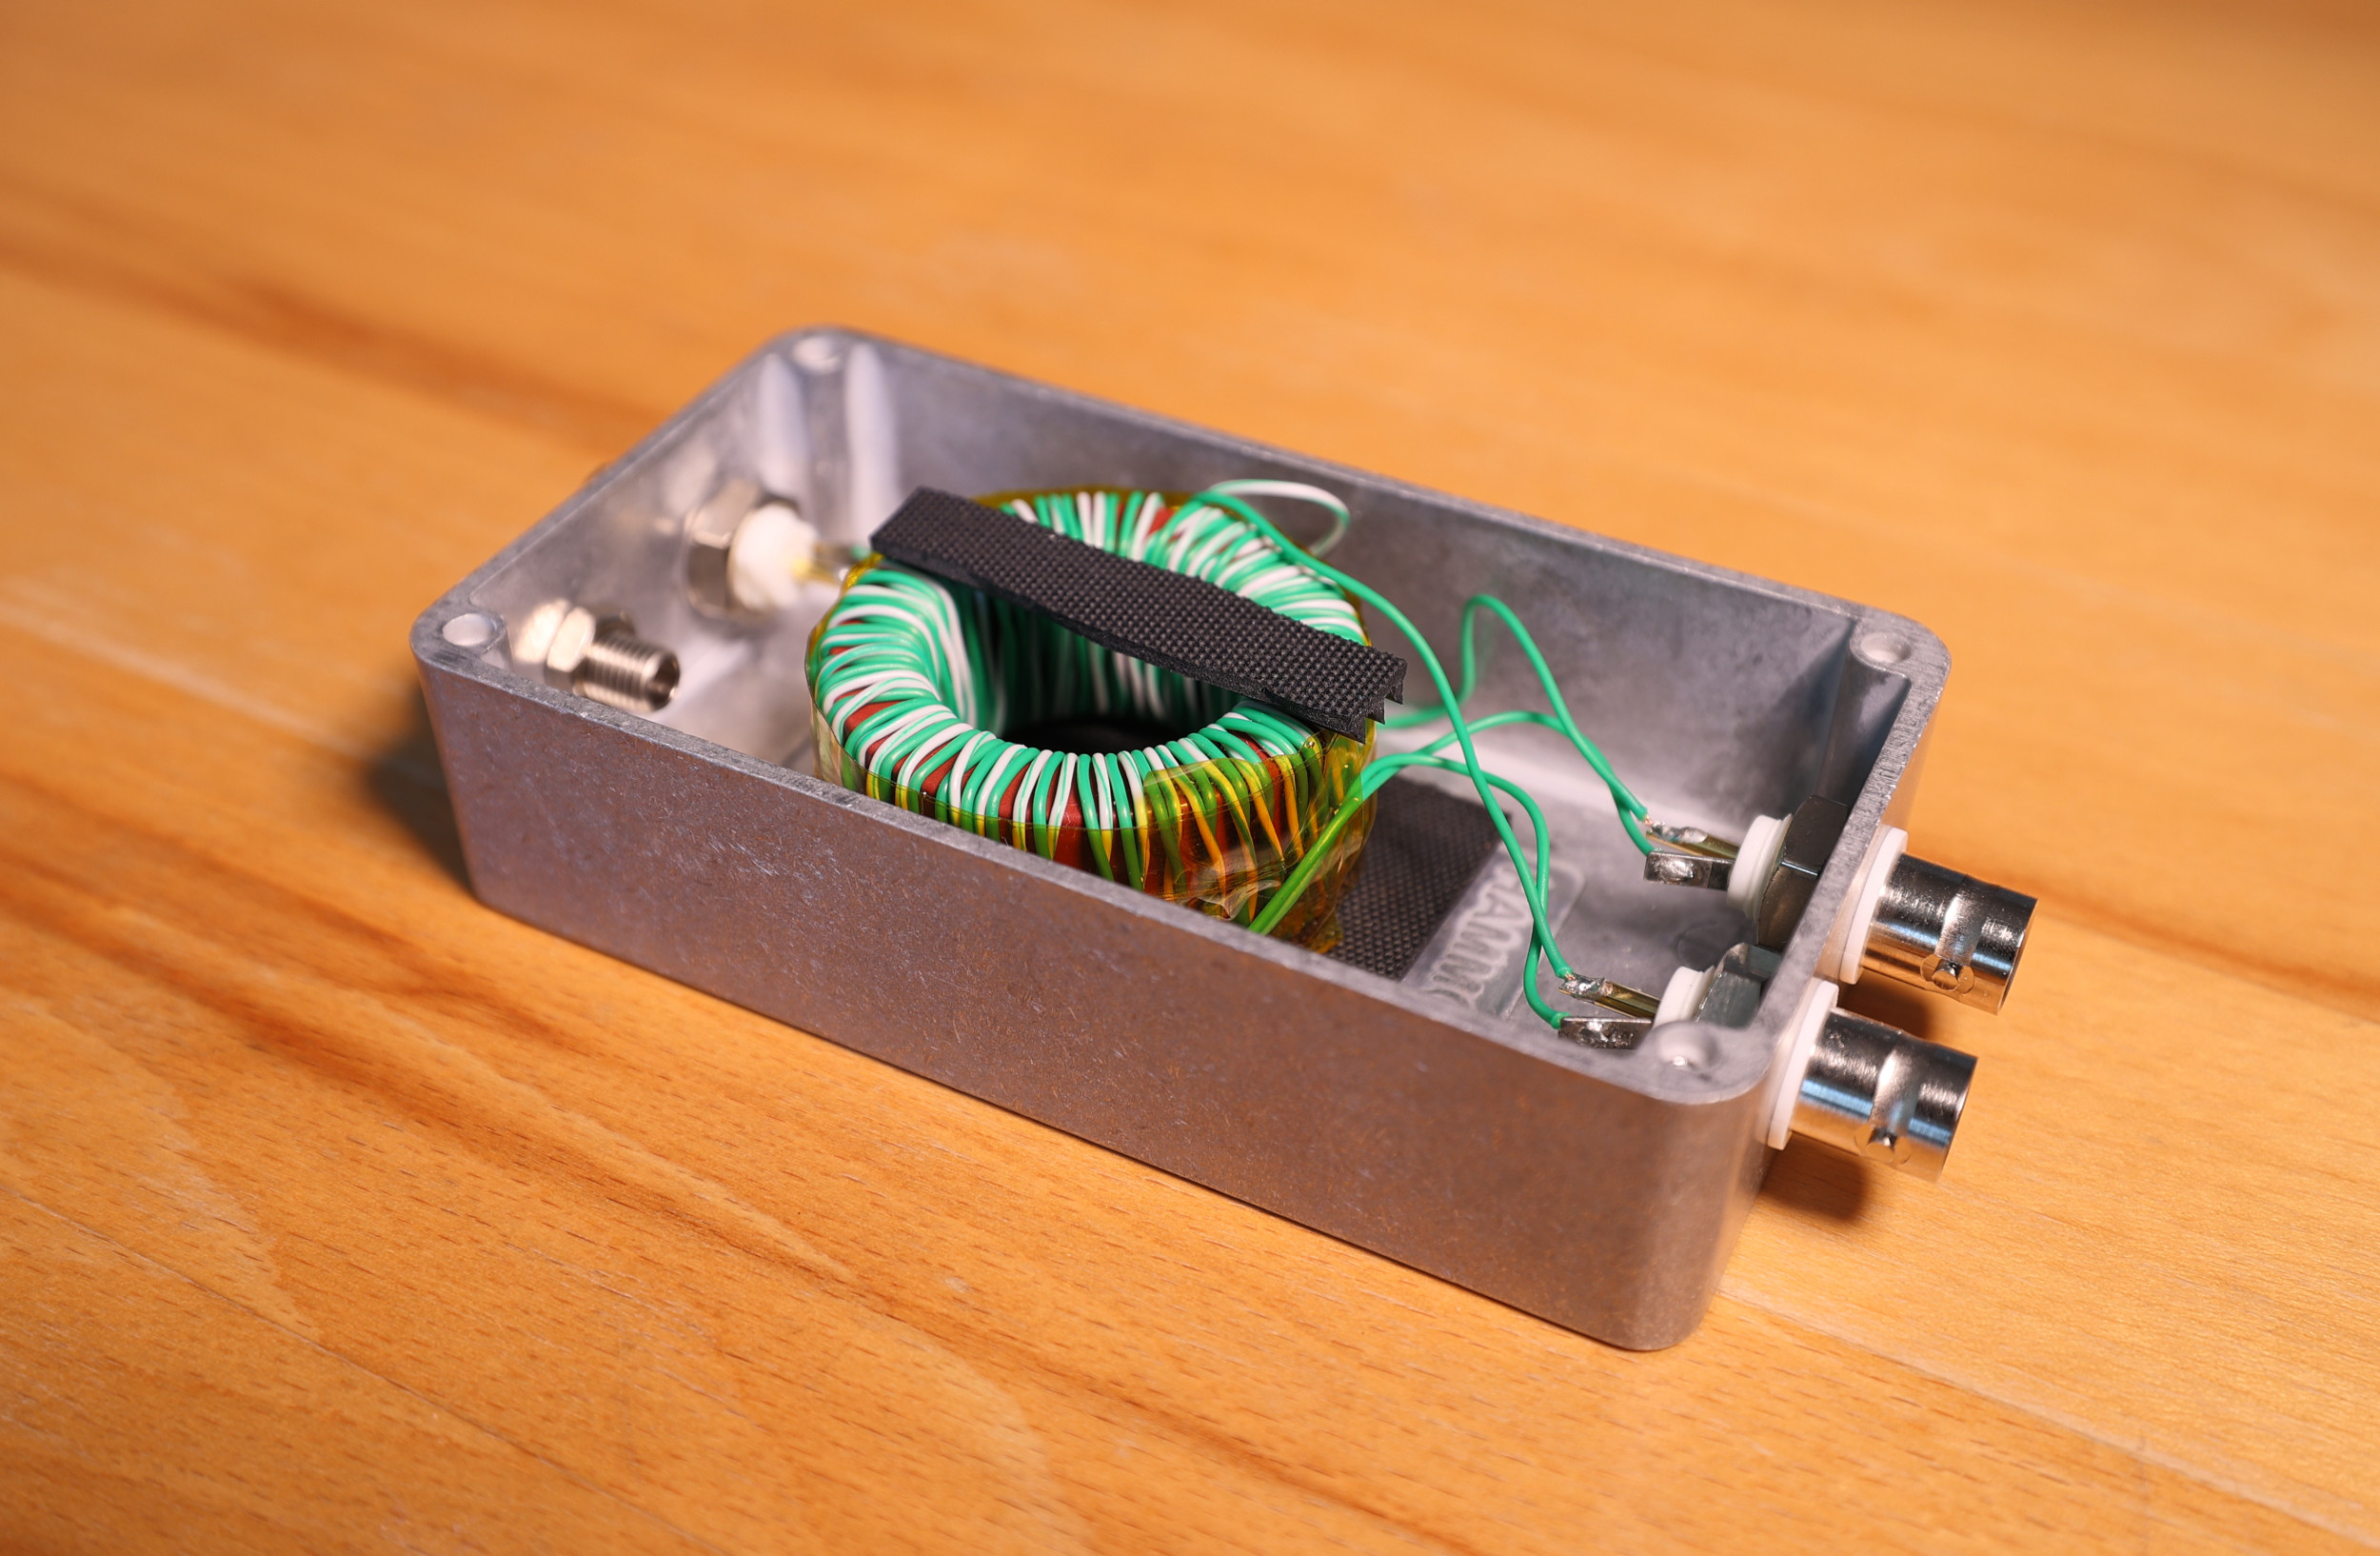
\includegraphics[width=0.75\textwidth]{../images/transformer_cropped_lowres.jpg}
    \caption{Photo of the finished injection transformer in its box. The black rubber is used to secure it in the box.}
    \label{fig:injection_transformer_assembled}
\end{figure}

After final assembly, the injection transformer was tested using a Picotest \device{Bode 100} VNA and also compared against a commercial Picotest \device{J2101A} 1:1 transformer.

\begin{figure}[hb!]
    \centering
    %% Creator: Matplotlib, PGF backend
%%
%% To include the figure in your LaTeX document, write
%%   \input{<filename>.pgf}
%%
%% Make sure the required packages are loaded in your preamble
%%   \usepackage{pgf}
%%
%% Also ensure that all the required font packages are loaded; for instance,
%% the lmodern package is sometimes necessary when using math font.
%%   \usepackage{lmodern}
%%
%% Figures using additional raster images can only be included by \input if
%% they are in the same directory as the main LaTeX file. For loading figures
%% from other directories you can use the `import` package
%%   \usepackage{import}
%%
%% and then include the figures with
%%   \import{<path to file>}{<filename>.pgf}
%%
%% Matplotlib used the following preamble
%%   \usepackage{siunitx}
%%   \usepackage{fontspec}
%%   \makeatletter\@ifpackageloaded{underscore}{}{\usepackage[strings]{underscore}}\makeatother
%%
\begingroup%
\makeatletter%
\begin{pgfpicture}%
\pgfpathrectangle{\pgfpointorigin}{\pgfqpoint{5.492126in}{3.394321in}}%
\pgfusepath{use as bounding box, clip}%
\begin{pgfscope}%
\pgfsetbuttcap%
\pgfsetmiterjoin%
\definecolor{currentfill}{rgb}{1.000000,1.000000,1.000000}%
\pgfsetfillcolor{currentfill}%
\pgfsetlinewidth{0.000000pt}%
\definecolor{currentstroke}{rgb}{1.000000,1.000000,1.000000}%
\pgfsetstrokecolor{currentstroke}%
\pgfsetdash{}{0pt}%
\pgfpathmoveto{\pgfqpoint{0.000000in}{0.000000in}}%
\pgfpathlineto{\pgfqpoint{5.492126in}{0.000000in}}%
\pgfpathlineto{\pgfqpoint{5.492126in}{3.394321in}}%
\pgfpathlineto{\pgfqpoint{0.000000in}{3.394321in}}%
\pgfpathlineto{\pgfqpoint{0.000000in}{0.000000in}}%
\pgfpathclose%
\pgfusepath{fill}%
\end{pgfscope}%
\begin{pgfscope}%
\pgfsetbuttcap%
\pgfsetmiterjoin%
\definecolor{currentfill}{rgb}{1.000000,1.000000,1.000000}%
\pgfsetfillcolor{currentfill}%
\pgfsetlinewidth{0.000000pt}%
\definecolor{currentstroke}{rgb}{0.000000,0.000000,0.000000}%
\pgfsetstrokecolor{currentstroke}%
\pgfsetstrokeopacity{0.000000}%
\pgfsetdash{}{0pt}%
\pgfpathmoveto{\pgfqpoint{0.634869in}{0.524170in}}%
\pgfpathlineto{\pgfqpoint{4.798449in}{0.524170in}}%
\pgfpathlineto{\pgfqpoint{4.798449in}{3.244321in}}%
\pgfpathlineto{\pgfqpoint{0.634869in}{3.244321in}}%
\pgfpathlineto{\pgfqpoint{0.634869in}{0.524170in}}%
\pgfpathclose%
\pgfusepath{fill}%
\end{pgfscope}%
\begin{pgfscope}%
\pgfpathrectangle{\pgfqpoint{0.634869in}{0.524170in}}{\pgfqpoint{4.163581in}{2.720151in}}%
\pgfusepath{clip}%
\pgfsetrectcap%
\pgfsetroundjoin%
\pgfsetlinewidth{0.803000pt}%
\definecolor{currentstroke}{rgb}{0.450000,0.450000,0.450000}%
\pgfsetstrokecolor{currentstroke}%
\pgfsetdash{}{0pt}%
\pgfpathmoveto{\pgfqpoint{1.315756in}{0.524170in}}%
\pgfpathlineto{\pgfqpoint{1.315756in}{3.244321in}}%
\pgfusepath{stroke}%
\end{pgfscope}%
\begin{pgfscope}%
\pgfsetbuttcap%
\pgfsetroundjoin%
\definecolor{currentfill}{rgb}{0.000000,0.000000,0.000000}%
\pgfsetfillcolor{currentfill}%
\pgfsetlinewidth{0.803000pt}%
\definecolor{currentstroke}{rgb}{0.000000,0.000000,0.000000}%
\pgfsetstrokecolor{currentstroke}%
\pgfsetdash{}{0pt}%
\pgfsys@defobject{currentmarker}{\pgfqpoint{0.000000in}{-0.048611in}}{\pgfqpoint{0.000000in}{0.000000in}}{%
\pgfpathmoveto{\pgfqpoint{0.000000in}{0.000000in}}%
\pgfpathlineto{\pgfqpoint{0.000000in}{-0.048611in}}%
\pgfusepath{stroke,fill}%
}%
\begin{pgfscope}%
\pgfsys@transformshift{1.315756in}{0.524170in}%
\pgfsys@useobject{currentmarker}{}%
\end{pgfscope}%
\end{pgfscope}%
\begin{pgfscope}%
\definecolor{textcolor}{rgb}{0.000000,0.000000,0.000000}%
\pgfsetstrokecolor{textcolor}%
\pgfsetfillcolor{textcolor}%
\pgftext[x=1.315756in,y=0.426948in,,top]{\color{textcolor}\rmfamily\fontsize{8.000000}{9.600000}\selectfont \(\displaystyle {10^{1}}\)}%
\end{pgfscope}%
\begin{pgfscope}%
\pgfpathrectangle{\pgfqpoint{0.634869in}{0.524170in}}{\pgfqpoint{4.163581in}{2.720151in}}%
\pgfusepath{clip}%
\pgfsetrectcap%
\pgfsetroundjoin%
\pgfsetlinewidth{0.803000pt}%
\definecolor{currentstroke}{rgb}{0.450000,0.450000,0.450000}%
\pgfsetstrokecolor{currentstroke}%
\pgfsetdash{}{0pt}%
\pgfpathmoveto{\pgfqpoint{2.299024in}{0.524170in}}%
\pgfpathlineto{\pgfqpoint{2.299024in}{3.244321in}}%
\pgfusepath{stroke}%
\end{pgfscope}%
\begin{pgfscope}%
\pgfsetbuttcap%
\pgfsetroundjoin%
\definecolor{currentfill}{rgb}{0.000000,0.000000,0.000000}%
\pgfsetfillcolor{currentfill}%
\pgfsetlinewidth{0.803000pt}%
\definecolor{currentstroke}{rgb}{0.000000,0.000000,0.000000}%
\pgfsetstrokecolor{currentstroke}%
\pgfsetdash{}{0pt}%
\pgfsys@defobject{currentmarker}{\pgfqpoint{0.000000in}{-0.048611in}}{\pgfqpoint{0.000000in}{0.000000in}}{%
\pgfpathmoveto{\pgfqpoint{0.000000in}{0.000000in}}%
\pgfpathlineto{\pgfqpoint{0.000000in}{-0.048611in}}%
\pgfusepath{stroke,fill}%
}%
\begin{pgfscope}%
\pgfsys@transformshift{2.299024in}{0.524170in}%
\pgfsys@useobject{currentmarker}{}%
\end{pgfscope}%
\end{pgfscope}%
\begin{pgfscope}%
\definecolor{textcolor}{rgb}{0.000000,0.000000,0.000000}%
\pgfsetstrokecolor{textcolor}%
\pgfsetfillcolor{textcolor}%
\pgftext[x=2.299024in,y=0.426948in,,top]{\color{textcolor}\rmfamily\fontsize{8.000000}{9.600000}\selectfont \(\displaystyle {10^{3}}\)}%
\end{pgfscope}%
\begin{pgfscope}%
\pgfpathrectangle{\pgfqpoint{0.634869in}{0.524170in}}{\pgfqpoint{4.163581in}{2.720151in}}%
\pgfusepath{clip}%
\pgfsetrectcap%
\pgfsetroundjoin%
\pgfsetlinewidth{0.803000pt}%
\definecolor{currentstroke}{rgb}{0.450000,0.450000,0.450000}%
\pgfsetstrokecolor{currentstroke}%
\pgfsetdash{}{0pt}%
\pgfpathmoveto{\pgfqpoint{3.282291in}{0.524170in}}%
\pgfpathlineto{\pgfqpoint{3.282291in}{3.244321in}}%
\pgfusepath{stroke}%
\end{pgfscope}%
\begin{pgfscope}%
\pgfsetbuttcap%
\pgfsetroundjoin%
\definecolor{currentfill}{rgb}{0.000000,0.000000,0.000000}%
\pgfsetfillcolor{currentfill}%
\pgfsetlinewidth{0.803000pt}%
\definecolor{currentstroke}{rgb}{0.000000,0.000000,0.000000}%
\pgfsetstrokecolor{currentstroke}%
\pgfsetdash{}{0pt}%
\pgfsys@defobject{currentmarker}{\pgfqpoint{0.000000in}{-0.048611in}}{\pgfqpoint{0.000000in}{0.000000in}}{%
\pgfpathmoveto{\pgfqpoint{0.000000in}{0.000000in}}%
\pgfpathlineto{\pgfqpoint{0.000000in}{-0.048611in}}%
\pgfusepath{stroke,fill}%
}%
\begin{pgfscope}%
\pgfsys@transformshift{3.282291in}{0.524170in}%
\pgfsys@useobject{currentmarker}{}%
\end{pgfscope}%
\end{pgfscope}%
\begin{pgfscope}%
\definecolor{textcolor}{rgb}{0.000000,0.000000,0.000000}%
\pgfsetstrokecolor{textcolor}%
\pgfsetfillcolor{textcolor}%
\pgftext[x=3.282291in,y=0.426948in,,top]{\color{textcolor}\rmfamily\fontsize{8.000000}{9.600000}\selectfont \(\displaystyle {10^{5}}\)}%
\end{pgfscope}%
\begin{pgfscope}%
\pgfpathrectangle{\pgfqpoint{0.634869in}{0.524170in}}{\pgfqpoint{4.163581in}{2.720151in}}%
\pgfusepath{clip}%
\pgfsetrectcap%
\pgfsetroundjoin%
\pgfsetlinewidth{0.803000pt}%
\definecolor{currentstroke}{rgb}{0.450000,0.450000,0.450000}%
\pgfsetstrokecolor{currentstroke}%
\pgfsetdash{}{0pt}%
\pgfpathmoveto{\pgfqpoint{4.265558in}{0.524170in}}%
\pgfpathlineto{\pgfqpoint{4.265558in}{3.244321in}}%
\pgfusepath{stroke}%
\end{pgfscope}%
\begin{pgfscope}%
\pgfsetbuttcap%
\pgfsetroundjoin%
\definecolor{currentfill}{rgb}{0.000000,0.000000,0.000000}%
\pgfsetfillcolor{currentfill}%
\pgfsetlinewidth{0.803000pt}%
\definecolor{currentstroke}{rgb}{0.000000,0.000000,0.000000}%
\pgfsetstrokecolor{currentstroke}%
\pgfsetdash{}{0pt}%
\pgfsys@defobject{currentmarker}{\pgfqpoint{0.000000in}{-0.048611in}}{\pgfqpoint{0.000000in}{0.000000in}}{%
\pgfpathmoveto{\pgfqpoint{0.000000in}{0.000000in}}%
\pgfpathlineto{\pgfqpoint{0.000000in}{-0.048611in}}%
\pgfusepath{stroke,fill}%
}%
\begin{pgfscope}%
\pgfsys@transformshift{4.265558in}{0.524170in}%
\pgfsys@useobject{currentmarker}{}%
\end{pgfscope}%
\end{pgfscope}%
\begin{pgfscope}%
\definecolor{textcolor}{rgb}{0.000000,0.000000,0.000000}%
\pgfsetstrokecolor{textcolor}%
\pgfsetfillcolor{textcolor}%
\pgftext[x=4.265558in,y=0.426948in,,top]{\color{textcolor}\rmfamily\fontsize{8.000000}{9.600000}\selectfont \(\displaystyle {10^{7}}\)}%
\end{pgfscope}%
\begin{pgfscope}%
\definecolor{textcolor}{rgb}{0.000000,0.000000,0.000000}%
\pgfsetstrokecolor{textcolor}%
\pgfsetfillcolor{textcolor}%
\pgftext[x=2.716659in,y=0.271531in,,top]{\color{textcolor}\rmfamily\fontsize{10.000000}{12.000000}\selectfont Frequency in \unit{\Hz}}%
\end{pgfscope}%
\begin{pgfscope}%
\pgfpathrectangle{\pgfqpoint{0.634869in}{0.524170in}}{\pgfqpoint{4.163581in}{2.720151in}}%
\pgfusepath{clip}%
\pgfsetrectcap%
\pgfsetroundjoin%
\pgfsetlinewidth{0.803000pt}%
\definecolor{currentstroke}{rgb}{0.450000,0.450000,0.450000}%
\pgfsetstrokecolor{currentstroke}%
\pgfsetdash{}{0pt}%
\pgfpathmoveto{\pgfqpoint{0.634869in}{0.536473in}}%
\pgfpathlineto{\pgfqpoint{4.798449in}{0.536473in}}%
\pgfusepath{stroke}%
\end{pgfscope}%
\begin{pgfscope}%
\pgfsetbuttcap%
\pgfsetroundjoin%
\definecolor{currentfill}{rgb}{0.000000,0.000000,0.000000}%
\pgfsetfillcolor{currentfill}%
\pgfsetlinewidth{0.803000pt}%
\definecolor{currentstroke}{rgb}{0.000000,0.000000,0.000000}%
\pgfsetstrokecolor{currentstroke}%
\pgfsetdash{}{0pt}%
\pgfsys@defobject{currentmarker}{\pgfqpoint{-0.048611in}{0.000000in}}{\pgfqpoint{-0.000000in}{0.000000in}}{%
\pgfpathmoveto{\pgfqpoint{-0.000000in}{0.000000in}}%
\pgfpathlineto{\pgfqpoint{-0.048611in}{0.000000in}}%
\pgfusepath{stroke,fill}%
}%
\begin{pgfscope}%
\pgfsys@transformshift{0.634869in}{0.536473in}%
\pgfsys@useobject{currentmarker}{}%
\end{pgfscope}%
\end{pgfscope}%
\begin{pgfscope}%
\definecolor{textcolor}{rgb}{0.000000,0.000000,0.000000}%
\pgfsetstrokecolor{textcolor}%
\pgfsetfillcolor{textcolor}%
\pgftext[x=0.327767in, y=0.497918in, left, base]{\color{textcolor}\rmfamily\fontsize{8.000000}{9.600000}\selectfont \(\displaystyle {\ensuremath{-}40}\)}%
\end{pgfscope}%
\begin{pgfscope}%
\pgfpathrectangle{\pgfqpoint{0.634869in}{0.524170in}}{\pgfqpoint{4.163581in}{2.720151in}}%
\pgfusepath{clip}%
\pgfsetrectcap%
\pgfsetroundjoin%
\pgfsetlinewidth{0.803000pt}%
\definecolor{currentstroke}{rgb}{0.450000,0.450000,0.450000}%
\pgfsetstrokecolor{currentstroke}%
\pgfsetdash{}{0pt}%
\pgfpathmoveto{\pgfqpoint{0.634869in}{0.859322in}}%
\pgfpathlineto{\pgfqpoint{4.798449in}{0.859322in}}%
\pgfusepath{stroke}%
\end{pgfscope}%
\begin{pgfscope}%
\pgfsetbuttcap%
\pgfsetroundjoin%
\definecolor{currentfill}{rgb}{0.000000,0.000000,0.000000}%
\pgfsetfillcolor{currentfill}%
\pgfsetlinewidth{0.803000pt}%
\definecolor{currentstroke}{rgb}{0.000000,0.000000,0.000000}%
\pgfsetstrokecolor{currentstroke}%
\pgfsetdash{}{0pt}%
\pgfsys@defobject{currentmarker}{\pgfqpoint{-0.048611in}{0.000000in}}{\pgfqpoint{-0.000000in}{0.000000in}}{%
\pgfpathmoveto{\pgfqpoint{-0.000000in}{0.000000in}}%
\pgfpathlineto{\pgfqpoint{-0.048611in}{0.000000in}}%
\pgfusepath{stroke,fill}%
}%
\begin{pgfscope}%
\pgfsys@transformshift{0.634869in}{0.859322in}%
\pgfsys@useobject{currentmarker}{}%
\end{pgfscope}%
\end{pgfscope}%
\begin{pgfscope}%
\definecolor{textcolor}{rgb}{0.000000,0.000000,0.000000}%
\pgfsetstrokecolor{textcolor}%
\pgfsetfillcolor{textcolor}%
\pgftext[x=0.327767in, y=0.820767in, left, base]{\color{textcolor}\rmfamily\fontsize{8.000000}{9.600000}\selectfont \(\displaystyle {\ensuremath{-}35}\)}%
\end{pgfscope}%
\begin{pgfscope}%
\pgfpathrectangle{\pgfqpoint{0.634869in}{0.524170in}}{\pgfqpoint{4.163581in}{2.720151in}}%
\pgfusepath{clip}%
\pgfsetrectcap%
\pgfsetroundjoin%
\pgfsetlinewidth{0.803000pt}%
\definecolor{currentstroke}{rgb}{0.450000,0.450000,0.450000}%
\pgfsetstrokecolor{currentstroke}%
\pgfsetdash{}{0pt}%
\pgfpathmoveto{\pgfqpoint{0.634869in}{1.182171in}}%
\pgfpathlineto{\pgfqpoint{4.798449in}{1.182171in}}%
\pgfusepath{stroke}%
\end{pgfscope}%
\begin{pgfscope}%
\pgfsetbuttcap%
\pgfsetroundjoin%
\definecolor{currentfill}{rgb}{0.000000,0.000000,0.000000}%
\pgfsetfillcolor{currentfill}%
\pgfsetlinewidth{0.803000pt}%
\definecolor{currentstroke}{rgb}{0.000000,0.000000,0.000000}%
\pgfsetstrokecolor{currentstroke}%
\pgfsetdash{}{0pt}%
\pgfsys@defobject{currentmarker}{\pgfqpoint{-0.048611in}{0.000000in}}{\pgfqpoint{-0.000000in}{0.000000in}}{%
\pgfpathmoveto{\pgfqpoint{-0.000000in}{0.000000in}}%
\pgfpathlineto{\pgfqpoint{-0.048611in}{0.000000in}}%
\pgfusepath{stroke,fill}%
}%
\begin{pgfscope}%
\pgfsys@transformshift{0.634869in}{1.182171in}%
\pgfsys@useobject{currentmarker}{}%
\end{pgfscope}%
\end{pgfscope}%
\begin{pgfscope}%
\definecolor{textcolor}{rgb}{0.000000,0.000000,0.000000}%
\pgfsetstrokecolor{textcolor}%
\pgfsetfillcolor{textcolor}%
\pgftext[x=0.327767in, y=1.143616in, left, base]{\color{textcolor}\rmfamily\fontsize{8.000000}{9.600000}\selectfont \(\displaystyle {\ensuremath{-}30}\)}%
\end{pgfscope}%
\begin{pgfscope}%
\pgfpathrectangle{\pgfqpoint{0.634869in}{0.524170in}}{\pgfqpoint{4.163581in}{2.720151in}}%
\pgfusepath{clip}%
\pgfsetrectcap%
\pgfsetroundjoin%
\pgfsetlinewidth{0.803000pt}%
\definecolor{currentstroke}{rgb}{0.450000,0.450000,0.450000}%
\pgfsetstrokecolor{currentstroke}%
\pgfsetdash{}{0pt}%
\pgfpathmoveto{\pgfqpoint{0.634869in}{1.505020in}}%
\pgfpathlineto{\pgfqpoint{4.798449in}{1.505020in}}%
\pgfusepath{stroke}%
\end{pgfscope}%
\begin{pgfscope}%
\pgfsetbuttcap%
\pgfsetroundjoin%
\definecolor{currentfill}{rgb}{0.000000,0.000000,0.000000}%
\pgfsetfillcolor{currentfill}%
\pgfsetlinewidth{0.803000pt}%
\definecolor{currentstroke}{rgb}{0.000000,0.000000,0.000000}%
\pgfsetstrokecolor{currentstroke}%
\pgfsetdash{}{0pt}%
\pgfsys@defobject{currentmarker}{\pgfqpoint{-0.048611in}{0.000000in}}{\pgfqpoint{-0.000000in}{0.000000in}}{%
\pgfpathmoveto{\pgfqpoint{-0.000000in}{0.000000in}}%
\pgfpathlineto{\pgfqpoint{-0.048611in}{0.000000in}}%
\pgfusepath{stroke,fill}%
}%
\begin{pgfscope}%
\pgfsys@transformshift{0.634869in}{1.505020in}%
\pgfsys@useobject{currentmarker}{}%
\end{pgfscope}%
\end{pgfscope}%
\begin{pgfscope}%
\definecolor{textcolor}{rgb}{0.000000,0.000000,0.000000}%
\pgfsetstrokecolor{textcolor}%
\pgfsetfillcolor{textcolor}%
\pgftext[x=0.327767in, y=1.466464in, left, base]{\color{textcolor}\rmfamily\fontsize{8.000000}{9.600000}\selectfont \(\displaystyle {\ensuremath{-}25}\)}%
\end{pgfscope}%
\begin{pgfscope}%
\pgfpathrectangle{\pgfqpoint{0.634869in}{0.524170in}}{\pgfqpoint{4.163581in}{2.720151in}}%
\pgfusepath{clip}%
\pgfsetrectcap%
\pgfsetroundjoin%
\pgfsetlinewidth{0.803000pt}%
\definecolor{currentstroke}{rgb}{0.450000,0.450000,0.450000}%
\pgfsetstrokecolor{currentstroke}%
\pgfsetdash{}{0pt}%
\pgfpathmoveto{\pgfqpoint{0.634869in}{1.827869in}}%
\pgfpathlineto{\pgfqpoint{4.798449in}{1.827869in}}%
\pgfusepath{stroke}%
\end{pgfscope}%
\begin{pgfscope}%
\pgfsetbuttcap%
\pgfsetroundjoin%
\definecolor{currentfill}{rgb}{0.000000,0.000000,0.000000}%
\pgfsetfillcolor{currentfill}%
\pgfsetlinewidth{0.803000pt}%
\definecolor{currentstroke}{rgb}{0.000000,0.000000,0.000000}%
\pgfsetstrokecolor{currentstroke}%
\pgfsetdash{}{0pt}%
\pgfsys@defobject{currentmarker}{\pgfqpoint{-0.048611in}{0.000000in}}{\pgfqpoint{-0.000000in}{0.000000in}}{%
\pgfpathmoveto{\pgfqpoint{-0.000000in}{0.000000in}}%
\pgfpathlineto{\pgfqpoint{-0.048611in}{0.000000in}}%
\pgfusepath{stroke,fill}%
}%
\begin{pgfscope}%
\pgfsys@transformshift{0.634869in}{1.827869in}%
\pgfsys@useobject{currentmarker}{}%
\end{pgfscope}%
\end{pgfscope}%
\begin{pgfscope}%
\definecolor{textcolor}{rgb}{0.000000,0.000000,0.000000}%
\pgfsetstrokecolor{textcolor}%
\pgfsetfillcolor{textcolor}%
\pgftext[x=0.327767in, y=1.789313in, left, base]{\color{textcolor}\rmfamily\fontsize{8.000000}{9.600000}\selectfont \(\displaystyle {\ensuremath{-}20}\)}%
\end{pgfscope}%
\begin{pgfscope}%
\pgfpathrectangle{\pgfqpoint{0.634869in}{0.524170in}}{\pgfqpoint{4.163581in}{2.720151in}}%
\pgfusepath{clip}%
\pgfsetrectcap%
\pgfsetroundjoin%
\pgfsetlinewidth{0.803000pt}%
\definecolor{currentstroke}{rgb}{0.450000,0.450000,0.450000}%
\pgfsetstrokecolor{currentstroke}%
\pgfsetdash{}{0pt}%
\pgfpathmoveto{\pgfqpoint{0.634869in}{2.150718in}}%
\pgfpathlineto{\pgfqpoint{4.798449in}{2.150718in}}%
\pgfusepath{stroke}%
\end{pgfscope}%
\begin{pgfscope}%
\pgfsetbuttcap%
\pgfsetroundjoin%
\definecolor{currentfill}{rgb}{0.000000,0.000000,0.000000}%
\pgfsetfillcolor{currentfill}%
\pgfsetlinewidth{0.803000pt}%
\definecolor{currentstroke}{rgb}{0.000000,0.000000,0.000000}%
\pgfsetstrokecolor{currentstroke}%
\pgfsetdash{}{0pt}%
\pgfsys@defobject{currentmarker}{\pgfqpoint{-0.048611in}{0.000000in}}{\pgfqpoint{-0.000000in}{0.000000in}}{%
\pgfpathmoveto{\pgfqpoint{-0.000000in}{0.000000in}}%
\pgfpathlineto{\pgfqpoint{-0.048611in}{0.000000in}}%
\pgfusepath{stroke,fill}%
}%
\begin{pgfscope}%
\pgfsys@transformshift{0.634869in}{2.150718in}%
\pgfsys@useobject{currentmarker}{}%
\end{pgfscope}%
\end{pgfscope}%
\begin{pgfscope}%
\definecolor{textcolor}{rgb}{0.000000,0.000000,0.000000}%
\pgfsetstrokecolor{textcolor}%
\pgfsetfillcolor{textcolor}%
\pgftext[x=0.327767in, y=2.112162in, left, base]{\color{textcolor}\rmfamily\fontsize{8.000000}{9.600000}\selectfont \(\displaystyle {\ensuremath{-}15}\)}%
\end{pgfscope}%
\begin{pgfscope}%
\pgfpathrectangle{\pgfqpoint{0.634869in}{0.524170in}}{\pgfqpoint{4.163581in}{2.720151in}}%
\pgfusepath{clip}%
\pgfsetrectcap%
\pgfsetroundjoin%
\pgfsetlinewidth{0.803000pt}%
\definecolor{currentstroke}{rgb}{0.450000,0.450000,0.450000}%
\pgfsetstrokecolor{currentstroke}%
\pgfsetdash{}{0pt}%
\pgfpathmoveto{\pgfqpoint{0.634869in}{2.473567in}}%
\pgfpathlineto{\pgfqpoint{4.798449in}{2.473567in}}%
\pgfusepath{stroke}%
\end{pgfscope}%
\begin{pgfscope}%
\pgfsetbuttcap%
\pgfsetroundjoin%
\definecolor{currentfill}{rgb}{0.000000,0.000000,0.000000}%
\pgfsetfillcolor{currentfill}%
\pgfsetlinewidth{0.803000pt}%
\definecolor{currentstroke}{rgb}{0.000000,0.000000,0.000000}%
\pgfsetstrokecolor{currentstroke}%
\pgfsetdash{}{0pt}%
\pgfsys@defobject{currentmarker}{\pgfqpoint{-0.048611in}{0.000000in}}{\pgfqpoint{-0.000000in}{0.000000in}}{%
\pgfpathmoveto{\pgfqpoint{-0.000000in}{0.000000in}}%
\pgfpathlineto{\pgfqpoint{-0.048611in}{0.000000in}}%
\pgfusepath{stroke,fill}%
}%
\begin{pgfscope}%
\pgfsys@transformshift{0.634869in}{2.473567in}%
\pgfsys@useobject{currentmarker}{}%
\end{pgfscope}%
\end{pgfscope}%
\begin{pgfscope}%
\definecolor{textcolor}{rgb}{0.000000,0.000000,0.000000}%
\pgfsetstrokecolor{textcolor}%
\pgfsetfillcolor{textcolor}%
\pgftext[x=0.327767in, y=2.435011in, left, base]{\color{textcolor}\rmfamily\fontsize{8.000000}{9.600000}\selectfont \(\displaystyle {\ensuremath{-}10}\)}%
\end{pgfscope}%
\begin{pgfscope}%
\pgfpathrectangle{\pgfqpoint{0.634869in}{0.524170in}}{\pgfqpoint{4.163581in}{2.720151in}}%
\pgfusepath{clip}%
\pgfsetrectcap%
\pgfsetroundjoin%
\pgfsetlinewidth{0.803000pt}%
\definecolor{currentstroke}{rgb}{0.450000,0.450000,0.450000}%
\pgfsetstrokecolor{currentstroke}%
\pgfsetdash{}{0pt}%
\pgfpathmoveto{\pgfqpoint{0.634869in}{2.796416in}}%
\pgfpathlineto{\pgfqpoint{4.798449in}{2.796416in}}%
\pgfusepath{stroke}%
\end{pgfscope}%
\begin{pgfscope}%
\pgfsetbuttcap%
\pgfsetroundjoin%
\definecolor{currentfill}{rgb}{0.000000,0.000000,0.000000}%
\pgfsetfillcolor{currentfill}%
\pgfsetlinewidth{0.803000pt}%
\definecolor{currentstroke}{rgb}{0.000000,0.000000,0.000000}%
\pgfsetstrokecolor{currentstroke}%
\pgfsetdash{}{0pt}%
\pgfsys@defobject{currentmarker}{\pgfqpoint{-0.048611in}{0.000000in}}{\pgfqpoint{-0.000000in}{0.000000in}}{%
\pgfpathmoveto{\pgfqpoint{-0.000000in}{0.000000in}}%
\pgfpathlineto{\pgfqpoint{-0.048611in}{0.000000in}}%
\pgfusepath{stroke,fill}%
}%
\begin{pgfscope}%
\pgfsys@transformshift{0.634869in}{2.796416in}%
\pgfsys@useobject{currentmarker}{}%
\end{pgfscope}%
\end{pgfscope}%
\begin{pgfscope}%
\definecolor{textcolor}{rgb}{0.000000,0.000000,0.000000}%
\pgfsetstrokecolor{textcolor}%
\pgfsetfillcolor{textcolor}%
\pgftext[x=0.386796in, y=2.757860in, left, base]{\color{textcolor}\rmfamily\fontsize{8.000000}{9.600000}\selectfont \(\displaystyle {\ensuremath{-}5}\)}%
\end{pgfscope}%
\begin{pgfscope}%
\pgfpathrectangle{\pgfqpoint{0.634869in}{0.524170in}}{\pgfqpoint{4.163581in}{2.720151in}}%
\pgfusepath{clip}%
\pgfsetrectcap%
\pgfsetroundjoin%
\pgfsetlinewidth{0.803000pt}%
\definecolor{currentstroke}{rgb}{0.450000,0.450000,0.450000}%
\pgfsetstrokecolor{currentstroke}%
\pgfsetdash{}{0pt}%
\pgfpathmoveto{\pgfqpoint{0.634869in}{3.119265in}}%
\pgfpathlineto{\pgfqpoint{4.798449in}{3.119265in}}%
\pgfusepath{stroke}%
\end{pgfscope}%
\begin{pgfscope}%
\pgfsetbuttcap%
\pgfsetroundjoin%
\definecolor{currentfill}{rgb}{0.000000,0.000000,0.000000}%
\pgfsetfillcolor{currentfill}%
\pgfsetlinewidth{0.803000pt}%
\definecolor{currentstroke}{rgb}{0.000000,0.000000,0.000000}%
\pgfsetstrokecolor{currentstroke}%
\pgfsetdash{}{0pt}%
\pgfsys@defobject{currentmarker}{\pgfqpoint{-0.048611in}{0.000000in}}{\pgfqpoint{-0.000000in}{0.000000in}}{%
\pgfpathmoveto{\pgfqpoint{-0.000000in}{0.000000in}}%
\pgfpathlineto{\pgfqpoint{-0.048611in}{0.000000in}}%
\pgfusepath{stroke,fill}%
}%
\begin{pgfscope}%
\pgfsys@transformshift{0.634869in}{3.119265in}%
\pgfsys@useobject{currentmarker}{}%
\end{pgfscope}%
\end{pgfscope}%
\begin{pgfscope}%
\definecolor{textcolor}{rgb}{0.000000,0.000000,0.000000}%
\pgfsetstrokecolor{textcolor}%
\pgfsetfillcolor{textcolor}%
\pgftext[x=0.478618in, y=3.080709in, left, base]{\color{textcolor}\rmfamily\fontsize{8.000000}{9.600000}\selectfont \(\displaystyle {0}\)}%
\end{pgfscope}%
\begin{pgfscope}%
\definecolor{textcolor}{rgb}{0.000000,0.000000,0.000000}%
\pgfsetstrokecolor{textcolor}%
\pgfsetfillcolor{textcolor}%
\pgftext[x=0.272211in,y=1.884245in,,bottom,rotate=90.000000]{\color{textcolor}\rmfamily\fontsize{10.000000}{12.000000}\selectfont Magnitude in \unit{\dB}}%
\end{pgfscope}%
\begin{pgfscope}%
\pgfpathrectangle{\pgfqpoint{0.634869in}{0.524170in}}{\pgfqpoint{4.163581in}{2.720151in}}%
\pgfusepath{clip}%
\pgfsetrectcap%
\pgfsetroundjoin%
\pgfsetlinewidth{1.003750pt}%
\definecolor{currentstroke}{rgb}{0.003922,0.450980,0.698039}%
\pgfsetstrokecolor{currentstroke}%
\pgfsetstrokeopacity{0.700000}%
\pgfsetdash{}{0pt}%
\pgfpathmoveto{\pgfqpoint{0.824122in}{1.898699in}}%
\pgfpathlineto{\pgfqpoint{0.843048in}{1.948076in}}%
\pgfpathlineto{\pgfqpoint{0.956600in}{2.210112in}}%
\pgfpathlineto{\pgfqpoint{0.966063in}{2.227420in}}%
\pgfpathlineto{\pgfqpoint{0.975525in}{2.251305in}}%
\pgfpathlineto{\pgfqpoint{1.013376in}{2.330127in}}%
\pgfpathlineto{\pgfqpoint{1.051227in}{2.401495in}}%
\pgfpathlineto{\pgfqpoint{1.089078in}{2.463947in}}%
\pgfpathlineto{\pgfqpoint{1.117466in}{2.506708in}}%
\pgfpathlineto{\pgfqpoint{1.136391in}{2.531796in}}%
\pgfpathlineto{\pgfqpoint{1.155316in}{2.555170in}}%
\pgfpathlineto{\pgfqpoint{1.174242in}{2.577186in}}%
\pgfpathlineto{\pgfqpoint{1.202630in}{2.605007in}}%
\pgfpathlineto{\pgfqpoint{1.221555in}{2.621335in}}%
\pgfpathlineto{\pgfqpoint{1.249943in}{2.642107in}}%
\pgfpathlineto{\pgfqpoint{1.278331in}{2.659151in}}%
\pgfpathlineto{\pgfqpoint{1.306719in}{2.672983in}}%
\pgfpathlineto{\pgfqpoint{1.335107in}{2.684201in}}%
\pgfpathlineto{\pgfqpoint{1.372958in}{2.695604in}}%
\pgfpathlineto{\pgfqpoint{1.410809in}{2.704027in}}%
\pgfpathlineto{\pgfqpoint{1.448659in}{2.709985in}}%
\pgfpathlineto{\pgfqpoint{1.495973in}{2.715261in}}%
\pgfpathlineto{\pgfqpoint{1.552749in}{2.719298in}}%
\pgfpathlineto{\pgfqpoint{1.637913in}{2.722563in}}%
\pgfpathlineto{\pgfqpoint{1.751465in}{2.724424in}}%
\pgfpathlineto{\pgfqpoint{1.978570in}{2.725414in}}%
\pgfpathlineto{\pgfqpoint{3.180331in}{2.724634in}}%
\pgfpathlineto{\pgfqpoint{3.388510in}{2.721874in}}%
\pgfpathlineto{\pgfqpoint{3.502062in}{2.716992in}}%
\pgfpathlineto{\pgfqpoint{3.558838in}{2.712325in}}%
\pgfpathlineto{\pgfqpoint{3.606151in}{2.706515in}}%
\pgfpathlineto{\pgfqpoint{3.653465in}{2.697960in}}%
\pgfpathlineto{\pgfqpoint{3.691315in}{2.688480in}}%
\pgfpathlineto{\pgfqpoint{3.719703in}{2.679502in}}%
\pgfpathlineto{\pgfqpoint{3.748091in}{2.668502in}}%
\pgfpathlineto{\pgfqpoint{3.776480in}{2.655180in}}%
\pgfpathlineto{\pgfqpoint{3.804868in}{2.639104in}}%
\pgfpathlineto{\pgfqpoint{3.833256in}{2.619912in}}%
\pgfpathlineto{\pgfqpoint{3.861644in}{2.597403in}}%
\pgfpathlineto{\pgfqpoint{3.890032in}{2.571186in}}%
\pgfpathlineto{\pgfqpoint{3.918420in}{2.541115in}}%
\pgfpathlineto{\pgfqpoint{3.946808in}{2.507065in}}%
\pgfpathlineto{\pgfqpoint{3.975196in}{2.469290in}}%
\pgfpathlineto{\pgfqpoint{4.003584in}{2.427607in}}%
\pgfpathlineto{\pgfqpoint{4.041435in}{2.366751in}}%
\pgfpathlineto{\pgfqpoint{4.079285in}{2.300393in}}%
\pgfpathlineto{\pgfqpoint{4.126599in}{2.211465in}}%
\pgfpathlineto{\pgfqpoint{4.173912in}{2.117555in}}%
\pgfpathlineto{\pgfqpoint{4.249614in}{1.961729in}}%
\pgfpathlineto{\pgfqpoint{4.278002in}{1.898113in}}%
\pgfpathlineto{\pgfqpoint{4.287464in}{1.873783in}}%
\pgfpathlineto{\pgfqpoint{4.296927in}{1.845906in}}%
\pgfpathlineto{\pgfqpoint{4.306390in}{1.810522in}}%
\pgfpathlineto{\pgfqpoint{4.315852in}{1.761595in}}%
\pgfpathlineto{\pgfqpoint{4.325315in}{1.687245in}}%
\pgfpathlineto{\pgfqpoint{4.334778in}{1.567018in}}%
\pgfpathlineto{\pgfqpoint{4.344241in}{1.367083in}}%
\pgfpathlineto{\pgfqpoint{4.353703in}{1.040449in}}%
\pgfpathlineto{\pgfqpoint{4.363166in}{0.647813in}}%
\pgfpathlineto{\pgfqpoint{4.372629in}{0.808707in}}%
\pgfpathlineto{\pgfqpoint{4.382091in}{1.035656in}}%
\pgfpathlineto{\pgfqpoint{4.391554in}{1.163229in}}%
\pgfpathlineto{\pgfqpoint{4.401017in}{1.238197in}}%
\pgfpathlineto{\pgfqpoint{4.410479in}{1.283978in}}%
\pgfpathlineto{\pgfqpoint{4.419942in}{1.314037in}}%
\pgfpathlineto{\pgfqpoint{4.429405in}{1.335912in}}%
\pgfpathlineto{\pgfqpoint{4.457793in}{1.388861in}}%
\pgfpathlineto{\pgfqpoint{4.467255in}{1.413411in}}%
\pgfpathlineto{\pgfqpoint{4.476718in}{1.444673in}}%
\pgfpathlineto{\pgfqpoint{4.486181in}{1.488352in}}%
\pgfpathlineto{\pgfqpoint{4.495643in}{1.547517in}}%
\pgfpathlineto{\pgfqpoint{4.505106in}{1.627771in}}%
\pgfpathlineto{\pgfqpoint{4.514569in}{1.738663in}}%
\pgfpathlineto{\pgfqpoint{4.524032in}{1.891542in}}%
\pgfpathlineto{\pgfqpoint{4.533494in}{2.092984in}}%
\pgfpathlineto{\pgfqpoint{4.542957in}{2.261632in}}%
\pgfpathlineto{\pgfqpoint{4.552420in}{2.169754in}}%
\pgfpathlineto{\pgfqpoint{4.561882in}{1.965790in}}%
\pgfpathlineto{\pgfqpoint{4.571345in}{1.806856in}}%
\pgfpathlineto{\pgfqpoint{4.580808in}{1.712941in}}%
\pgfpathlineto{\pgfqpoint{4.599733in}{1.852102in}}%
\pgfpathlineto{\pgfqpoint{4.609196in}{1.740056in}}%
\pgfpathlineto{\pgfqpoint{4.609196in}{1.740056in}}%
\pgfusepath{stroke}%
\end{pgfscope}%
\begin{pgfscope}%
\pgfpathrectangle{\pgfqpoint{0.634869in}{0.524170in}}{\pgfqpoint{4.163581in}{2.720151in}}%
\pgfusepath{clip}%
\pgfsetrectcap%
\pgfsetroundjoin%
\pgfsetlinewidth{1.003750pt}%
\definecolor{currentstroke}{rgb}{0.870588,0.560784,0.019608}%
\pgfsetstrokecolor{currentstroke}%
\pgfsetstrokeopacity{0.700000}%
\pgfsetdash{}{0pt}%
\pgfpathmoveto{\pgfqpoint{0.824122in}{1.891317in}}%
\pgfpathlineto{\pgfqpoint{0.843048in}{1.941613in}}%
\pgfpathlineto{\pgfqpoint{0.928212in}{2.143284in}}%
\pgfpathlineto{\pgfqpoint{0.966063in}{2.227549in}}%
\pgfpathlineto{\pgfqpoint{1.032301in}{2.361184in}}%
\pgfpathlineto{\pgfqpoint{1.060689in}{2.413034in}}%
\pgfpathlineto{\pgfqpoint{1.089078in}{2.460506in}}%
\pgfpathlineto{\pgfqpoint{1.117466in}{2.503503in}}%
\pgfpathlineto{\pgfqpoint{1.145854in}{2.541536in}}%
\pgfpathlineto{\pgfqpoint{1.164779in}{2.564501in}}%
\pgfpathlineto{\pgfqpoint{1.193167in}{2.594085in}}%
\pgfpathlineto{\pgfqpoint{1.221555in}{2.619538in}}%
\pgfpathlineto{\pgfqpoint{1.240480in}{2.634054in}}%
\pgfpathlineto{\pgfqpoint{1.259406in}{2.646834in}}%
\pgfpathlineto{\pgfqpoint{1.287794in}{2.663047in}}%
\pgfpathlineto{\pgfqpoint{1.316182in}{2.676182in}}%
\pgfpathlineto{\pgfqpoint{1.344570in}{2.686782in}}%
\pgfpathlineto{\pgfqpoint{1.372958in}{2.695115in}}%
\pgfpathlineto{\pgfqpoint{1.410809in}{2.703664in}}%
\pgfpathlineto{\pgfqpoint{1.448659in}{2.709836in}}%
\pgfpathlineto{\pgfqpoint{1.495973in}{2.715154in}}%
\pgfpathlineto{\pgfqpoint{1.543286in}{2.718708in}}%
\pgfpathlineto{\pgfqpoint{1.628450in}{2.722342in}}%
\pgfpathlineto{\pgfqpoint{1.751465in}{2.724498in}}%
\pgfpathlineto{\pgfqpoint{1.988032in}{2.725521in}}%
\pgfpathlineto{\pgfqpoint{2.924838in}{2.725518in}}%
\pgfpathlineto{\pgfqpoint{3.350659in}{2.722583in}}%
\pgfpathlineto{\pgfqpoint{3.435823in}{2.720000in}}%
\pgfpathlineto{\pgfqpoint{3.511524in}{2.715415in}}%
\pgfpathlineto{\pgfqpoint{3.558838in}{2.710830in}}%
\pgfpathlineto{\pgfqpoint{3.606151in}{2.704048in}}%
\pgfpathlineto{\pgfqpoint{3.644002in}{2.696397in}}%
\pgfpathlineto{\pgfqpoint{3.681853in}{2.686053in}}%
\pgfpathlineto{\pgfqpoint{3.710241in}{2.676134in}}%
\pgfpathlineto{\pgfqpoint{3.738629in}{2.663736in}}%
\pgfpathlineto{\pgfqpoint{3.767017in}{2.648461in}}%
\pgfpathlineto{\pgfqpoint{3.795405in}{2.629727in}}%
\pgfpathlineto{\pgfqpoint{3.814330in}{2.615020in}}%
\pgfpathlineto{\pgfqpoint{3.833256in}{2.598211in}}%
\pgfpathlineto{\pgfqpoint{3.852181in}{2.579230in}}%
\pgfpathlineto{\pgfqpoint{3.871106in}{2.557627in}}%
\pgfpathlineto{\pgfqpoint{3.890032in}{2.533238in}}%
\pgfpathlineto{\pgfqpoint{3.908957in}{2.505715in}}%
\pgfpathlineto{\pgfqpoint{3.927882in}{2.474641in}}%
\pgfpathlineto{\pgfqpoint{3.946808in}{2.439547in}}%
\pgfpathlineto{\pgfqpoint{3.965733in}{2.400012in}}%
\pgfpathlineto{\pgfqpoint{3.984659in}{2.355275in}}%
\pgfpathlineto{\pgfqpoint{4.003584in}{2.304218in}}%
\pgfpathlineto{\pgfqpoint{4.022509in}{2.245415in}}%
\pgfpathlineto{\pgfqpoint{4.041435in}{2.177081in}}%
\pgfpathlineto{\pgfqpoint{4.060360in}{2.095668in}}%
\pgfpathlineto{\pgfqpoint{4.079285in}{1.996153in}}%
\pgfpathlineto{\pgfqpoint{4.088748in}{1.937055in}}%
\pgfpathlineto{\pgfqpoint{4.098211in}{1.869353in}}%
\pgfpathlineto{\pgfqpoint{4.107673in}{1.790165in}}%
\pgfpathlineto{\pgfqpoint{4.117136in}{1.696094in}}%
\pgfpathlineto{\pgfqpoint{4.126599in}{1.580476in}}%
\pgfpathlineto{\pgfqpoint{4.136061in}{1.432354in}}%
\pgfpathlineto{\pgfqpoint{4.145524in}{1.236090in}}%
\pgfpathlineto{\pgfqpoint{4.154987in}{0.988614in}}%
\pgfpathlineto{\pgfqpoint{4.164450in}{0.914912in}}%
\pgfpathlineto{\pgfqpoint{4.183375in}{1.420554in}}%
\pgfpathlineto{\pgfqpoint{4.192838in}{1.615434in}}%
\pgfpathlineto{\pgfqpoint{4.202300in}{1.772811in}}%
\pgfpathlineto{\pgfqpoint{4.211763in}{1.905929in}}%
\pgfpathlineto{\pgfqpoint{4.230688in}{2.128706in}}%
\pgfpathlineto{\pgfqpoint{4.249614in}{2.320931in}}%
\pgfpathlineto{\pgfqpoint{4.315852in}{2.946686in}}%
\pgfpathlineto{\pgfqpoint{4.325315in}{3.026455in}}%
\pgfpathlineto{\pgfqpoint{4.334778in}{3.088335in}}%
\pgfpathlineto{\pgfqpoint{4.344241in}{3.120677in}}%
\pgfpathlineto{\pgfqpoint{4.353703in}{3.116279in}}%
\pgfpathlineto{\pgfqpoint{4.363166in}{3.080057in}}%
\pgfpathlineto{\pgfqpoint{4.372629in}{3.024406in}}%
\pgfpathlineto{\pgfqpoint{4.419942in}{2.709767in}}%
\pgfpathlineto{\pgfqpoint{4.438867in}{2.603281in}}%
\pgfpathlineto{\pgfqpoint{4.457793in}{2.507890in}}%
\pgfpathlineto{\pgfqpoint{4.486181in}{2.379340in}}%
\pgfpathlineto{\pgfqpoint{4.505106in}{2.301983in}}%
\pgfpathlineto{\pgfqpoint{4.514569in}{2.267835in}}%
\pgfpathlineto{\pgfqpoint{4.533494in}{2.204246in}}%
\pgfpathlineto{\pgfqpoint{4.542957in}{2.089344in}}%
\pgfpathlineto{\pgfqpoint{4.552420in}{1.746048in}}%
\pgfpathlineto{\pgfqpoint{4.561882in}{1.568092in}}%
\pgfpathlineto{\pgfqpoint{4.571345in}{1.497836in}}%
\pgfpathlineto{\pgfqpoint{4.580808in}{1.653135in}}%
\pgfpathlineto{\pgfqpoint{4.590270in}{1.998004in}}%
\pgfpathlineto{\pgfqpoint{4.609196in}{1.712046in}}%
\pgfpathlineto{\pgfqpoint{4.609196in}{1.712046in}}%
\pgfusepath{stroke}%
\end{pgfscope}%
\begin{pgfscope}%
\pgfpathrectangle{\pgfqpoint{0.634869in}{0.524170in}}{\pgfqpoint{4.163581in}{2.720151in}}%
\pgfusepath{clip}%
\pgfsetrectcap%
\pgfsetroundjoin%
\pgfsetlinewidth{1.003750pt}%
\definecolor{currentstroke}{rgb}{0.007843,0.619608,0.450980}%
\pgfsetstrokecolor{currentstroke}%
\pgfsetstrokeopacity{0.700000}%
\pgfsetdash{}{0pt}%
\pgfpathmoveto{\pgfqpoint{0.824122in}{2.716581in}}%
\pgfpathlineto{\pgfqpoint{0.843048in}{2.753246in}}%
\pgfpathlineto{\pgfqpoint{0.880899in}{2.817942in}}%
\pgfpathlineto{\pgfqpoint{0.937675in}{2.900015in}}%
\pgfpathlineto{\pgfqpoint{0.956600in}{2.923584in}}%
\pgfpathlineto{\pgfqpoint{0.984988in}{2.955389in}}%
\pgfpathlineto{\pgfqpoint{1.013376in}{2.982409in}}%
\pgfpathlineto{\pgfqpoint{1.041764in}{3.005170in}}%
\pgfpathlineto{\pgfqpoint{1.060689in}{3.018136in}}%
\pgfpathlineto{\pgfqpoint{1.079615in}{3.029741in}}%
\pgfpathlineto{\pgfqpoint{1.108003in}{3.044119in}}%
\pgfpathlineto{\pgfqpoint{1.136391in}{3.055940in}}%
\pgfpathlineto{\pgfqpoint{1.164779in}{3.065416in}}%
\pgfpathlineto{\pgfqpoint{1.202630in}{3.075057in}}%
\pgfpathlineto{\pgfqpoint{1.240480in}{3.082195in}}%
\pgfpathlineto{\pgfqpoint{1.287794in}{3.088532in}}%
\pgfpathlineto{\pgfqpoint{1.344570in}{3.093573in}}%
\pgfpathlineto{\pgfqpoint{1.420271in}{3.097734in}}%
\pgfpathlineto{\pgfqpoint{1.533824in}{3.101350in}}%
\pgfpathlineto{\pgfqpoint{1.723077in}{3.104936in}}%
\pgfpathlineto{\pgfqpoint{1.874480in}{3.106020in}}%
\pgfpathlineto{\pgfqpoint{3.388510in}{3.106173in}}%
\pgfpathlineto{\pgfqpoint{3.615614in}{3.104240in}}%
\pgfpathlineto{\pgfqpoint{3.700778in}{3.102055in}}%
\pgfpathlineto{\pgfqpoint{3.785942in}{3.097959in}}%
\pgfpathlineto{\pgfqpoint{3.852181in}{3.092662in}}%
\pgfpathlineto{\pgfqpoint{3.899494in}{3.087107in}}%
\pgfpathlineto{\pgfqpoint{3.946808in}{3.079301in}}%
\pgfpathlineto{\pgfqpoint{3.984659in}{3.071149in}}%
\pgfpathlineto{\pgfqpoint{4.022509in}{3.060422in}}%
\pgfpathlineto{\pgfqpoint{4.050897in}{3.050314in}}%
\pgfpathlineto{\pgfqpoint{4.079285in}{3.037944in}}%
\pgfpathlineto{\pgfqpoint{4.107673in}{3.022832in}}%
\pgfpathlineto{\pgfqpoint{4.126599in}{3.010948in}}%
\pgfpathlineto{\pgfqpoint{4.145524in}{2.997506in}}%
\pgfpathlineto{\pgfqpoint{4.173912in}{2.973602in}}%
\pgfpathlineto{\pgfqpoint{4.192838in}{2.954953in}}%
\pgfpathlineto{\pgfqpoint{4.211763in}{2.933902in}}%
\pgfpathlineto{\pgfqpoint{4.230688in}{2.909869in}}%
\pgfpathlineto{\pgfqpoint{4.249614in}{2.882595in}}%
\pgfpathlineto{\pgfqpoint{4.268539in}{2.851753in}}%
\pgfpathlineto{\pgfqpoint{4.287464in}{2.816171in}}%
\pgfpathlineto{\pgfqpoint{4.306390in}{2.775046in}}%
\pgfpathlineto{\pgfqpoint{4.325315in}{2.726297in}}%
\pgfpathlineto{\pgfqpoint{4.334778in}{2.697983in}}%
\pgfpathlineto{\pgfqpoint{4.344241in}{2.666032in}}%
\pgfpathlineto{\pgfqpoint{4.353703in}{2.629190in}}%
\pgfpathlineto{\pgfqpoint{4.363166in}{2.585357in}}%
\pgfpathlineto{\pgfqpoint{4.372629in}{2.530790in}}%
\pgfpathlineto{\pgfqpoint{4.382091in}{2.458242in}}%
\pgfpathlineto{\pgfqpoint{4.391554in}{2.351329in}}%
\pgfpathlineto{\pgfqpoint{4.401017in}{2.165224in}}%
\pgfpathlineto{\pgfqpoint{4.410479in}{1.762502in}}%
\pgfpathlineto{\pgfqpoint{4.419942in}{2.152221in}}%
\pgfpathlineto{\pgfqpoint{4.429405in}{2.765570in}}%
\pgfpathlineto{\pgfqpoint{4.438867in}{2.982956in}}%
\pgfpathlineto{\pgfqpoint{4.448330in}{2.941028in}}%
\pgfpathlineto{\pgfqpoint{4.457793in}{2.864696in}}%
\pgfpathlineto{\pgfqpoint{4.467255in}{2.797914in}}%
\pgfpathlineto{\pgfqpoint{4.476718in}{2.742025in}}%
\pgfpathlineto{\pgfqpoint{4.495643in}{2.651060in}}%
\pgfpathlineto{\pgfqpoint{4.514569in}{2.575813in}}%
\pgfpathlineto{\pgfqpoint{4.542957in}{2.476772in}}%
\pgfpathlineto{\pgfqpoint{4.599733in}{2.289021in}}%
\pgfpathlineto{\pgfqpoint{4.609196in}{2.257679in}}%
\pgfpathlineto{\pgfqpoint{4.609196in}{2.257679in}}%
\pgfusepath{stroke}%
\end{pgfscope}%
\begin{pgfscope}%
\pgfsetrectcap%
\pgfsetmiterjoin%
\pgfsetlinewidth{0.803000pt}%
\definecolor{currentstroke}{rgb}{0.000000,0.000000,0.000000}%
\pgfsetstrokecolor{currentstroke}%
\pgfsetdash{}{0pt}%
\pgfpathmoveto{\pgfqpoint{0.634869in}{0.524170in}}%
\pgfpathlineto{\pgfqpoint{0.634869in}{3.244321in}}%
\pgfusepath{stroke}%
\end{pgfscope}%
\begin{pgfscope}%
\pgfsetrectcap%
\pgfsetmiterjoin%
\pgfsetlinewidth{0.803000pt}%
\definecolor{currentstroke}{rgb}{0.000000,0.000000,0.000000}%
\pgfsetstrokecolor{currentstroke}%
\pgfsetdash{}{0pt}%
\pgfpathmoveto{\pgfqpoint{4.798449in}{0.524170in}}%
\pgfpathlineto{\pgfqpoint{4.798449in}{3.244321in}}%
\pgfusepath{stroke}%
\end{pgfscope}%
\begin{pgfscope}%
\pgfsetrectcap%
\pgfsetmiterjoin%
\pgfsetlinewidth{0.803000pt}%
\definecolor{currentstroke}{rgb}{0.000000,0.000000,0.000000}%
\pgfsetstrokecolor{currentstroke}%
\pgfsetdash{}{0pt}%
\pgfpathmoveto{\pgfqpoint{0.634869in}{0.524170in}}%
\pgfpathlineto{\pgfqpoint{4.798449in}{0.524170in}}%
\pgfusepath{stroke}%
\end{pgfscope}%
\begin{pgfscope}%
\pgfsetrectcap%
\pgfsetmiterjoin%
\pgfsetlinewidth{0.803000pt}%
\definecolor{currentstroke}{rgb}{0.000000,0.000000,0.000000}%
\pgfsetstrokecolor{currentstroke}%
\pgfsetdash{}{0pt}%
\pgfpathmoveto{\pgfqpoint{0.634869in}{3.244321in}}%
\pgfpathlineto{\pgfqpoint{4.798449in}{3.244321in}}%
\pgfusepath{stroke}%
\end{pgfscope}%
\begin{pgfscope}%
\pgfsetbuttcap%
\pgfsetroundjoin%
\definecolor{currentfill}{rgb}{0.000000,0.000000,0.000000}%
\pgfsetfillcolor{currentfill}%
\pgfsetlinewidth{0.803000pt}%
\definecolor{currentstroke}{rgb}{0.000000,0.000000,0.000000}%
\pgfsetstrokecolor{currentstroke}%
\pgfsetdash{}{0pt}%
\pgfsys@defobject{currentmarker}{\pgfqpoint{0.000000in}{0.000000in}}{\pgfqpoint{0.048611in}{0.000000in}}{%
\pgfpathmoveto{\pgfqpoint{0.000000in}{0.000000in}}%
\pgfpathlineto{\pgfqpoint{0.048611in}{0.000000in}}%
\pgfusepath{stroke,fill}%
}%
\begin{pgfscope}%
\pgfsys@transformshift{4.798449in}{0.858858in}%
\pgfsys@useobject{currentmarker}{}%
\end{pgfscope}%
\end{pgfscope}%
\begin{pgfscope}%
\definecolor{textcolor}{rgb}{0.000000,0.000000,0.000000}%
\pgfsetstrokecolor{textcolor}%
\pgfsetfillcolor{textcolor}%
\pgftext[x=4.895672in, y=0.820302in, left, base]{\color{textcolor}\rmfamily\fontsize{8.000000}{9.600000}\selectfont \(\displaystyle {\ensuremath{-}400}\)}%
\end{pgfscope}%
\begin{pgfscope}%
\pgfsetbuttcap%
\pgfsetroundjoin%
\definecolor{currentfill}{rgb}{0.000000,0.000000,0.000000}%
\pgfsetfillcolor{currentfill}%
\pgfsetlinewidth{0.803000pt}%
\definecolor{currentstroke}{rgb}{0.000000,0.000000,0.000000}%
\pgfsetstrokecolor{currentstroke}%
\pgfsetdash{}{0pt}%
\pgfsys@defobject{currentmarker}{\pgfqpoint{0.000000in}{0.000000in}}{\pgfqpoint{0.048611in}{0.000000in}}{%
\pgfpathmoveto{\pgfqpoint{0.000000in}{0.000000in}}%
\pgfpathlineto{\pgfqpoint{0.048611in}{0.000000in}}%
\pgfusepath{stroke,fill}%
}%
\begin{pgfscope}%
\pgfsys@transformshift{4.798449in}{1.327637in}%
\pgfsys@useobject{currentmarker}{}%
\end{pgfscope}%
\end{pgfscope}%
\begin{pgfscope}%
\definecolor{textcolor}{rgb}{0.000000,0.000000,0.000000}%
\pgfsetstrokecolor{textcolor}%
\pgfsetfillcolor{textcolor}%
\pgftext[x=4.895672in, y=1.289082in, left, base]{\color{textcolor}\rmfamily\fontsize{8.000000}{9.600000}\selectfont \(\displaystyle {\ensuremath{-}300}\)}%
\end{pgfscope}%
\begin{pgfscope}%
\pgfsetbuttcap%
\pgfsetroundjoin%
\definecolor{currentfill}{rgb}{0.000000,0.000000,0.000000}%
\pgfsetfillcolor{currentfill}%
\pgfsetlinewidth{0.803000pt}%
\definecolor{currentstroke}{rgb}{0.000000,0.000000,0.000000}%
\pgfsetstrokecolor{currentstroke}%
\pgfsetdash{}{0pt}%
\pgfsys@defobject{currentmarker}{\pgfqpoint{0.000000in}{0.000000in}}{\pgfqpoint{0.048611in}{0.000000in}}{%
\pgfpathmoveto{\pgfqpoint{0.000000in}{0.000000in}}%
\pgfpathlineto{\pgfqpoint{0.048611in}{0.000000in}}%
\pgfusepath{stroke,fill}%
}%
\begin{pgfscope}%
\pgfsys@transformshift{4.798449in}{1.796417in}%
\pgfsys@useobject{currentmarker}{}%
\end{pgfscope}%
\end{pgfscope}%
\begin{pgfscope}%
\definecolor{textcolor}{rgb}{0.000000,0.000000,0.000000}%
\pgfsetstrokecolor{textcolor}%
\pgfsetfillcolor{textcolor}%
\pgftext[x=4.895672in, y=1.757862in, left, base]{\color{textcolor}\rmfamily\fontsize{8.000000}{9.600000}\selectfont \(\displaystyle {\ensuremath{-}200}\)}%
\end{pgfscope}%
\begin{pgfscope}%
\pgfsetbuttcap%
\pgfsetroundjoin%
\definecolor{currentfill}{rgb}{0.000000,0.000000,0.000000}%
\pgfsetfillcolor{currentfill}%
\pgfsetlinewidth{0.803000pt}%
\definecolor{currentstroke}{rgb}{0.000000,0.000000,0.000000}%
\pgfsetstrokecolor{currentstroke}%
\pgfsetdash{}{0pt}%
\pgfsys@defobject{currentmarker}{\pgfqpoint{0.000000in}{0.000000in}}{\pgfqpoint{0.048611in}{0.000000in}}{%
\pgfpathmoveto{\pgfqpoint{0.000000in}{0.000000in}}%
\pgfpathlineto{\pgfqpoint{0.048611in}{0.000000in}}%
\pgfusepath{stroke,fill}%
}%
\begin{pgfscope}%
\pgfsys@transformshift{4.798449in}{2.265197in}%
\pgfsys@useobject{currentmarker}{}%
\end{pgfscope}%
\end{pgfscope}%
\begin{pgfscope}%
\definecolor{textcolor}{rgb}{0.000000,0.000000,0.000000}%
\pgfsetstrokecolor{textcolor}%
\pgfsetfillcolor{textcolor}%
\pgftext[x=4.895672in, y=2.226642in, left, base]{\color{textcolor}\rmfamily\fontsize{8.000000}{9.600000}\selectfont \(\displaystyle {\ensuremath{-}100}\)}%
\end{pgfscope}%
\begin{pgfscope}%
\pgfsetbuttcap%
\pgfsetroundjoin%
\definecolor{currentfill}{rgb}{0.000000,0.000000,0.000000}%
\pgfsetfillcolor{currentfill}%
\pgfsetlinewidth{0.803000pt}%
\definecolor{currentstroke}{rgb}{0.000000,0.000000,0.000000}%
\pgfsetstrokecolor{currentstroke}%
\pgfsetdash{}{0pt}%
\pgfsys@defobject{currentmarker}{\pgfqpoint{0.000000in}{0.000000in}}{\pgfqpoint{0.048611in}{0.000000in}}{%
\pgfpathmoveto{\pgfqpoint{0.000000in}{0.000000in}}%
\pgfpathlineto{\pgfqpoint{0.048611in}{0.000000in}}%
\pgfusepath{stroke,fill}%
}%
\begin{pgfscope}%
\pgfsys@transformshift{4.798449in}{2.733977in}%
\pgfsys@useobject{currentmarker}{}%
\end{pgfscope}%
\end{pgfscope}%
\begin{pgfscope}%
\definecolor{textcolor}{rgb}{0.000000,0.000000,0.000000}%
\pgfsetstrokecolor{textcolor}%
\pgfsetfillcolor{textcolor}%
\pgftext[x=4.895672in, y=2.695422in, left, base]{\color{textcolor}\rmfamily\fontsize{8.000000}{9.600000}\selectfont \(\displaystyle {0}\)}%
\end{pgfscope}%
\begin{pgfscope}%
\pgfsetbuttcap%
\pgfsetroundjoin%
\definecolor{currentfill}{rgb}{0.000000,0.000000,0.000000}%
\pgfsetfillcolor{currentfill}%
\pgfsetlinewidth{0.803000pt}%
\definecolor{currentstroke}{rgb}{0.000000,0.000000,0.000000}%
\pgfsetstrokecolor{currentstroke}%
\pgfsetdash{}{0pt}%
\pgfsys@defobject{currentmarker}{\pgfqpoint{0.000000in}{0.000000in}}{\pgfqpoint{0.048611in}{0.000000in}}{%
\pgfpathmoveto{\pgfqpoint{0.000000in}{0.000000in}}%
\pgfpathlineto{\pgfqpoint{0.048611in}{0.000000in}}%
\pgfusepath{stroke,fill}%
}%
\begin{pgfscope}%
\pgfsys@transformshift{4.798449in}{3.202757in}%
\pgfsys@useobject{currentmarker}{}%
\end{pgfscope}%
\end{pgfscope}%
\begin{pgfscope}%
\definecolor{textcolor}{rgb}{0.000000,0.000000,0.000000}%
\pgfsetstrokecolor{textcolor}%
\pgfsetfillcolor{textcolor}%
\pgftext[x=4.895672in, y=3.164202in, left, base]{\color{textcolor}\rmfamily\fontsize{8.000000}{9.600000}\selectfont \(\displaystyle {100}\)}%
\end{pgfscope}%
\begin{pgfscope}%
\definecolor{textcolor}{rgb}{0.000000,0.000000,0.000000}%
\pgfsetstrokecolor{textcolor}%
\pgfsetfillcolor{textcolor}%
\pgftext[x=5.220135in,y=1.884245in,,top,rotate=90.000000]{\color{textcolor}\rmfamily\fontsize{10.000000}{12.000000}\selectfont Phase in \unit{\degree}}%
\end{pgfscope}%
\begin{pgfscope}%
\pgfpathrectangle{\pgfqpoint{0.634869in}{0.524170in}}{\pgfqpoint{4.163581in}{2.720151in}}%
\pgfusepath{clip}%
\pgfsetbuttcap%
\pgfsetroundjoin%
\pgfsetlinewidth{1.003750pt}%
\definecolor{currentstroke}{rgb}{0.003922,0.450980,0.698039}%
\pgfsetstrokecolor{currentstroke}%
\pgfsetstrokeopacity{0.700000}%
\pgfsetdash{{3.700000pt}{1.600000pt}}{0.000000pt}%
\pgfpathmoveto{\pgfqpoint{0.824122in}{2.247706in}}%
\pgfpathlineto{\pgfqpoint{0.880899in}{2.229502in}}%
\pgfpathlineto{\pgfqpoint{0.909287in}{2.219188in}}%
\pgfpathlineto{\pgfqpoint{0.947137in}{2.203630in}}%
\pgfpathlineto{\pgfqpoint{0.984988in}{2.185442in}}%
\pgfpathlineto{\pgfqpoint{1.022839in}{2.165441in}}%
\pgfpathlineto{\pgfqpoint{1.070152in}{2.138544in}}%
\pgfpathlineto{\pgfqpoint{1.155316in}{2.086273in}}%
\pgfpathlineto{\pgfqpoint{1.193167in}{2.062804in}}%
\pgfpathlineto{\pgfqpoint{1.249943in}{2.030227in}}%
\pgfpathlineto{\pgfqpoint{1.297257in}{2.006182in}}%
\pgfpathlineto{\pgfqpoint{1.335107in}{1.989175in}}%
\pgfpathlineto{\pgfqpoint{1.391883in}{1.967592in}}%
\pgfpathlineto{\pgfqpoint{1.429734in}{1.955576in}}%
\pgfpathlineto{\pgfqpoint{1.477048in}{1.943049in}}%
\pgfpathlineto{\pgfqpoint{1.524361in}{1.932725in}}%
\pgfpathlineto{\pgfqpoint{1.581137in}{1.922905in}}%
\pgfpathlineto{\pgfqpoint{1.637913in}{1.915321in}}%
\pgfpathlineto{\pgfqpoint{1.704152in}{1.908637in}}%
\pgfpathlineto{\pgfqpoint{1.779853in}{1.903132in}}%
\pgfpathlineto{\pgfqpoint{1.874480in}{1.898484in}}%
\pgfpathlineto{\pgfqpoint{1.997495in}{1.894819in}}%
\pgfpathlineto{\pgfqpoint{2.167823in}{1.892205in}}%
\pgfpathlineto{\pgfqpoint{2.442241in}{1.890470in}}%
\pgfpathlineto{\pgfqpoint{2.868062in}{1.888142in}}%
\pgfpathlineto{\pgfqpoint{3.057316in}{1.885167in}}%
\pgfpathlineto{\pgfqpoint{3.189793in}{1.881006in}}%
\pgfpathlineto{\pgfqpoint{3.303345in}{1.874742in}}%
\pgfpathlineto{\pgfqpoint{3.379047in}{1.868392in}}%
\pgfpathlineto{\pgfqpoint{3.445286in}{1.860744in}}%
\pgfpathlineto{\pgfqpoint{3.511524in}{1.850507in}}%
\pgfpathlineto{\pgfqpoint{3.558838in}{1.841170in}}%
\pgfpathlineto{\pgfqpoint{3.606151in}{1.829838in}}%
\pgfpathlineto{\pgfqpoint{3.653465in}{1.816181in}}%
\pgfpathlineto{\pgfqpoint{3.700778in}{1.799855in}}%
\pgfpathlineto{\pgfqpoint{3.738629in}{1.784816in}}%
\pgfpathlineto{\pgfqpoint{3.785942in}{1.763419in}}%
\pgfpathlineto{\pgfqpoint{3.833256in}{1.739297in}}%
\pgfpathlineto{\pgfqpoint{3.890032in}{1.707276in}}%
\pgfpathlineto{\pgfqpoint{3.975196in}{1.655695in}}%
\pgfpathlineto{\pgfqpoint{4.164450in}{1.538173in}}%
\pgfpathlineto{\pgfqpoint{4.192838in}{1.518266in}}%
\pgfpathlineto{\pgfqpoint{4.221226in}{1.495522in}}%
\pgfpathlineto{\pgfqpoint{4.240151in}{1.477458in}}%
\pgfpathlineto{\pgfqpoint{4.259076in}{1.455413in}}%
\pgfpathlineto{\pgfqpoint{4.268539in}{1.442218in}}%
\pgfpathlineto{\pgfqpoint{4.278002in}{1.426787in}}%
\pgfpathlineto{\pgfqpoint{4.287464in}{1.408587in}}%
\pgfpathlineto{\pgfqpoint{4.296927in}{1.386550in}}%
\pgfpathlineto{\pgfqpoint{4.306390in}{1.359315in}}%
\pgfpathlineto{\pgfqpoint{4.315852in}{1.325347in}}%
\pgfpathlineto{\pgfqpoint{4.325315in}{1.284485in}}%
\pgfpathlineto{\pgfqpoint{4.344241in}{1.194242in}}%
\pgfpathlineto{\pgfqpoint{4.353703in}{1.189814in}}%
\pgfpathlineto{\pgfqpoint{4.363166in}{1.350108in}}%
\pgfpathlineto{\pgfqpoint{4.372629in}{1.574575in}}%
\pgfpathlineto{\pgfqpoint{4.382091in}{1.618283in}}%
\pgfpathlineto{\pgfqpoint{4.391554in}{1.618031in}}%
\pgfpathlineto{\pgfqpoint{4.401017in}{1.607367in}}%
\pgfpathlineto{\pgfqpoint{4.429405in}{1.571418in}}%
\pgfpathlineto{\pgfqpoint{4.476718in}{1.516986in}}%
\pgfpathlineto{\pgfqpoint{4.486181in}{1.503873in}}%
\pgfpathlineto{\pgfqpoint{4.495643in}{1.487882in}}%
\pgfpathlineto{\pgfqpoint{4.505106in}{1.466964in}}%
\pgfpathlineto{\pgfqpoint{4.514569in}{1.438693in}}%
\pgfpathlineto{\pgfqpoint{4.524032in}{1.393588in}}%
\pgfpathlineto{\pgfqpoint{4.533494in}{1.308812in}}%
\pgfpathlineto{\pgfqpoint{4.542957in}{1.138606in}}%
\pgfpathlineto{\pgfqpoint{4.552420in}{0.941723in}}%
\pgfpathlineto{\pgfqpoint{4.561882in}{0.838774in}}%
\pgfpathlineto{\pgfqpoint{4.571345in}{0.797357in}}%
\pgfpathlineto{\pgfqpoint{4.580808in}{0.793932in}}%
\pgfpathlineto{\pgfqpoint{4.590270in}{0.810090in}}%
\pgfpathlineto{\pgfqpoint{4.599733in}{0.695159in}}%
\pgfpathlineto{\pgfqpoint{4.609196in}{0.647813in}}%
\pgfpathlineto{\pgfqpoint{4.609196in}{0.647813in}}%
\pgfusepath{stroke}%
\end{pgfscope}%
\begin{pgfscope}%
\pgfpathrectangle{\pgfqpoint{0.634869in}{0.524170in}}{\pgfqpoint{4.163581in}{2.720151in}}%
\pgfusepath{clip}%
\pgfsetbuttcap%
\pgfsetroundjoin%
\pgfsetlinewidth{1.003750pt}%
\definecolor{currentstroke}{rgb}{0.870588,0.560784,0.019608}%
\pgfsetstrokecolor{currentstroke}%
\pgfsetstrokeopacity{0.700000}%
\pgfsetdash{{3.700000pt}{1.600000pt}}{0.000000pt}%
\pgfpathmoveto{\pgfqpoint{0.824122in}{3.090884in}}%
\pgfpathlineto{\pgfqpoint{0.890361in}{3.070057in}}%
\pgfpathlineto{\pgfqpoint{0.928212in}{3.055158in}}%
\pgfpathlineto{\pgfqpoint{0.966063in}{3.038565in}}%
\pgfpathlineto{\pgfqpoint{1.003913in}{3.020530in}}%
\pgfpathlineto{\pgfqpoint{1.060689in}{2.988828in}}%
\pgfpathlineto{\pgfqpoint{1.155316in}{2.930848in}}%
\pgfpathlineto{\pgfqpoint{1.202630in}{2.902065in}}%
\pgfpathlineto{\pgfqpoint{1.240480in}{2.880263in}}%
\pgfpathlineto{\pgfqpoint{1.278331in}{2.860210in}}%
\pgfpathlineto{\pgfqpoint{1.316182in}{2.842101in}}%
\pgfpathlineto{\pgfqpoint{1.354033in}{2.826034in}}%
\pgfpathlineto{\pgfqpoint{1.391883in}{2.812009in}}%
\pgfpathlineto{\pgfqpoint{1.439197in}{2.797212in}}%
\pgfpathlineto{\pgfqpoint{1.486510in}{2.785079in}}%
\pgfpathlineto{\pgfqpoint{1.533824in}{2.775070in}}%
\pgfpathlineto{\pgfqpoint{1.600062in}{2.764282in}}%
\pgfpathlineto{\pgfqpoint{1.666301in}{2.756238in}}%
\pgfpathlineto{\pgfqpoint{1.742003in}{2.749607in}}%
\pgfpathlineto{\pgfqpoint{1.827167in}{2.744469in}}%
\pgfpathlineto{\pgfqpoint{1.931256in}{2.740410in}}%
\pgfpathlineto{\pgfqpoint{2.073197in}{2.737245in}}%
\pgfpathlineto{\pgfqpoint{2.290838in}{2.735032in}}%
\pgfpathlineto{\pgfqpoint{3.038390in}{2.729495in}}%
\pgfpathlineto{\pgfqpoint{3.180331in}{2.725354in}}%
\pgfpathlineto{\pgfqpoint{3.284420in}{2.720077in}}%
\pgfpathlineto{\pgfqpoint{3.369584in}{2.713502in}}%
\pgfpathlineto{\pgfqpoint{3.445286in}{2.705067in}}%
\pgfpathlineto{\pgfqpoint{3.502062in}{2.696622in}}%
\pgfpathlineto{\pgfqpoint{3.549375in}{2.687893in}}%
\pgfpathlineto{\pgfqpoint{3.606151in}{2.674804in}}%
\pgfpathlineto{\pgfqpoint{3.653465in}{2.661420in}}%
\pgfpathlineto{\pgfqpoint{3.700778in}{2.645485in}}%
\pgfpathlineto{\pgfqpoint{3.748091in}{2.626796in}}%
\pgfpathlineto{\pgfqpoint{3.785942in}{2.609901in}}%
\pgfpathlineto{\pgfqpoint{3.833256in}{2.586431in}}%
\pgfpathlineto{\pgfqpoint{3.890032in}{2.555529in}}%
\pgfpathlineto{\pgfqpoint{4.022509in}{2.481284in}}%
\pgfpathlineto{\pgfqpoint{4.050897in}{2.467794in}}%
\pgfpathlineto{\pgfqpoint{4.069823in}{2.460383in}}%
\pgfpathlineto{\pgfqpoint{4.088748in}{2.455306in}}%
\pgfpathlineto{\pgfqpoint{4.098211in}{2.454336in}}%
\pgfpathlineto{\pgfqpoint{4.107673in}{2.455164in}}%
\pgfpathlineto{\pgfqpoint{4.117136in}{2.458866in}}%
\pgfpathlineto{\pgfqpoint{4.126599in}{2.467486in}}%
\pgfpathlineto{\pgfqpoint{4.136061in}{2.485871in}}%
\pgfpathlineto{\pgfqpoint{4.145524in}{2.527452in}}%
\pgfpathlineto{\pgfqpoint{4.154987in}{2.634857in}}%
\pgfpathlineto{\pgfqpoint{4.164450in}{2.862103in}}%
\pgfpathlineto{\pgfqpoint{4.173912in}{3.022004in}}%
\pgfpathlineto{\pgfqpoint{4.183375in}{3.082579in}}%
\pgfpathlineto{\pgfqpoint{4.192838in}{3.107139in}}%
\pgfpathlineto{\pgfqpoint{4.202300in}{3.117427in}}%
\pgfpathlineto{\pgfqpoint{4.211763in}{3.120677in}}%
\pgfpathlineto{\pgfqpoint{4.221226in}{3.119746in}}%
\pgfpathlineto{\pgfqpoint{4.230688in}{3.115941in}}%
\pgfpathlineto{\pgfqpoint{4.240151in}{3.109784in}}%
\pgfpathlineto{\pgfqpoint{4.249614in}{3.101513in}}%
\pgfpathlineto{\pgfqpoint{4.259076in}{3.091082in}}%
\pgfpathlineto{\pgfqpoint{4.268539in}{3.078214in}}%
\pgfpathlineto{\pgfqpoint{4.278002in}{3.062409in}}%
\pgfpathlineto{\pgfqpoint{4.287464in}{3.042880in}}%
\pgfpathlineto{\pgfqpoint{4.296927in}{3.018487in}}%
\pgfpathlineto{\pgfqpoint{4.306390in}{2.987763in}}%
\pgfpathlineto{\pgfqpoint{4.315852in}{2.948695in}}%
\pgfpathlineto{\pgfqpoint{4.325315in}{2.899372in}}%
\pgfpathlineto{\pgfqpoint{4.334778in}{2.839449in}}%
\pgfpathlineto{\pgfqpoint{4.363166in}{2.640819in}}%
\pgfpathlineto{\pgfqpoint{4.372629in}{2.589469in}}%
\pgfpathlineto{\pgfqpoint{4.382091in}{2.548619in}}%
\pgfpathlineto{\pgfqpoint{4.391554in}{2.516252in}}%
\pgfpathlineto{\pgfqpoint{4.401017in}{2.490658in}}%
\pgfpathlineto{\pgfqpoint{4.410479in}{2.470125in}}%
\pgfpathlineto{\pgfqpoint{4.419942in}{2.453111in}}%
\pgfpathlineto{\pgfqpoint{4.438867in}{2.426487in}}%
\pgfpathlineto{\pgfqpoint{4.457793in}{2.406091in}}%
\pgfpathlineto{\pgfqpoint{4.505106in}{2.360452in}}%
\pgfpathlineto{\pgfqpoint{4.514569in}{2.348008in}}%
\pgfpathlineto{\pgfqpoint{4.524032in}{2.328799in}}%
\pgfpathlineto{\pgfqpoint{4.533494in}{2.291280in}}%
\pgfpathlineto{\pgfqpoint{4.542957in}{2.216479in}}%
\pgfpathlineto{\pgfqpoint{4.552420in}{2.206216in}}%
\pgfpathlineto{\pgfqpoint{4.561882in}{2.319301in}}%
\pgfpathlineto{\pgfqpoint{4.571345in}{2.418056in}}%
\pgfpathlineto{\pgfqpoint{4.580808in}{2.584001in}}%
\pgfpathlineto{\pgfqpoint{4.590270in}{2.468861in}}%
\pgfpathlineto{\pgfqpoint{4.599733in}{2.373408in}}%
\pgfpathlineto{\pgfqpoint{4.609196in}{2.350517in}}%
\pgfpathlineto{\pgfqpoint{4.609196in}{2.350517in}}%
\pgfusepath{stroke}%
\end{pgfscope}%
\begin{pgfscope}%
\pgfpathrectangle{\pgfqpoint{0.634869in}{0.524170in}}{\pgfqpoint{4.163581in}{2.720151in}}%
\pgfusepath{clip}%
\pgfsetbuttcap%
\pgfsetroundjoin%
\pgfsetlinewidth{1.003750pt}%
\definecolor{currentstroke}{rgb}{0.007843,0.619608,0.450980}%
\pgfsetstrokecolor{currentstroke}%
\pgfsetstrokeopacity{0.700000}%
\pgfsetdash{{3.700000pt}{1.600000pt}}{0.000000pt}%
\pgfpathmoveto{\pgfqpoint{0.824122in}{3.008986in}}%
\pgfpathlineto{\pgfqpoint{0.947137in}{2.937005in}}%
\pgfpathlineto{\pgfqpoint{1.051227in}{2.876039in}}%
\pgfpathlineto{\pgfqpoint{1.108003in}{2.847546in}}%
\pgfpathlineto{\pgfqpoint{1.145854in}{2.830901in}}%
\pgfpathlineto{\pgfqpoint{1.183704in}{2.816226in}}%
\pgfpathlineto{\pgfqpoint{1.231018in}{2.800666in}}%
\pgfpathlineto{\pgfqpoint{1.278331in}{2.787817in}}%
\pgfpathlineto{\pgfqpoint{1.325645in}{2.777274in}}%
\pgfpathlineto{\pgfqpoint{1.372958in}{2.768690in}}%
\pgfpathlineto{\pgfqpoint{1.429734in}{2.760495in}}%
\pgfpathlineto{\pgfqpoint{1.495973in}{2.753208in}}%
\pgfpathlineto{\pgfqpoint{1.571674in}{2.747113in}}%
\pgfpathlineto{\pgfqpoint{1.666301in}{2.741818in}}%
\pgfpathlineto{\pgfqpoint{1.789316in}{2.737359in}}%
\pgfpathlineto{\pgfqpoint{1.883943in}{2.735890in}}%
\pgfpathlineto{\pgfqpoint{2.139435in}{2.734571in}}%
\pgfpathlineto{\pgfqpoint{3.265495in}{2.730852in}}%
\pgfpathlineto{\pgfqpoint{3.397972in}{2.728223in}}%
\pgfpathlineto{\pgfqpoint{3.530450in}{2.723363in}}%
\pgfpathlineto{\pgfqpoint{3.625077in}{2.717591in}}%
\pgfpathlineto{\pgfqpoint{3.700778in}{2.710927in}}%
\pgfpathlineto{\pgfqpoint{3.767017in}{2.703071in}}%
\pgfpathlineto{\pgfqpoint{3.833256in}{2.692727in}}%
\pgfpathlineto{\pgfqpoint{3.890032in}{2.681308in}}%
\pgfpathlineto{\pgfqpoint{3.946808in}{2.667015in}}%
\pgfpathlineto{\pgfqpoint{3.994121in}{2.652418in}}%
\pgfpathlineto{\pgfqpoint{4.031972in}{2.638741in}}%
\pgfpathlineto{\pgfqpoint{4.069823in}{2.623103in}}%
\pgfpathlineto{\pgfqpoint{4.107673in}{2.605348in}}%
\pgfpathlineto{\pgfqpoint{4.145524in}{2.585487in}}%
\pgfpathlineto{\pgfqpoint{4.192838in}{2.557741in}}%
\pgfpathlineto{\pgfqpoint{4.240151in}{2.527157in}}%
\pgfpathlineto{\pgfqpoint{4.296927in}{2.487454in}}%
\pgfpathlineto{\pgfqpoint{4.344241in}{2.452073in}}%
\pgfpathlineto{\pgfqpoint{4.382091in}{2.422023in}}%
\pgfpathlineto{\pgfqpoint{4.391554in}{2.416964in}}%
\pgfpathlineto{\pgfqpoint{4.401017in}{2.424236in}}%
\pgfpathlineto{\pgfqpoint{4.410479in}{2.540513in}}%
\pgfpathlineto{\pgfqpoint{4.419942in}{2.929090in}}%
\pgfpathlineto{\pgfqpoint{4.429405in}{2.871544in}}%
\pgfpathlineto{\pgfqpoint{4.438867in}{2.697849in}}%
\pgfpathlineto{\pgfqpoint{4.448330in}{2.578684in}}%
\pgfpathlineto{\pgfqpoint{4.457793in}{2.520131in}}%
\pgfpathlineto{\pgfqpoint{4.467255in}{2.486201in}}%
\pgfpathlineto{\pgfqpoint{4.476718in}{2.464187in}}%
\pgfpathlineto{\pgfqpoint{4.486181in}{2.448418in}}%
\pgfpathlineto{\pgfqpoint{4.495643in}{2.436114in}}%
\pgfpathlineto{\pgfqpoint{4.514569in}{2.417914in}}%
\pgfpathlineto{\pgfqpoint{4.533494in}{2.403956in}}%
\pgfpathlineto{\pgfqpoint{4.552420in}{2.391960in}}%
\pgfpathlineto{\pgfqpoint{4.580808in}{2.377448in}}%
\pgfpathlineto{\pgfqpoint{4.609196in}{2.365017in}}%
\pgfpathlineto{\pgfqpoint{4.609196in}{2.365017in}}%
\pgfusepath{stroke}%
\end{pgfscope}%
\begin{pgfscope}%
\pgfsetrectcap%
\pgfsetmiterjoin%
\pgfsetlinewidth{0.803000pt}%
\definecolor{currentstroke}{rgb}{0.000000,0.000000,0.000000}%
\pgfsetstrokecolor{currentstroke}%
\pgfsetdash{}{0pt}%
\pgfpathmoveto{\pgfqpoint{0.634869in}{0.524170in}}%
\pgfpathlineto{\pgfqpoint{0.634869in}{3.244321in}}%
\pgfusepath{stroke}%
\end{pgfscope}%
\begin{pgfscope}%
\pgfsetrectcap%
\pgfsetmiterjoin%
\pgfsetlinewidth{0.803000pt}%
\definecolor{currentstroke}{rgb}{0.000000,0.000000,0.000000}%
\pgfsetstrokecolor{currentstroke}%
\pgfsetdash{}{0pt}%
\pgfpathmoveto{\pgfqpoint{4.798449in}{0.524170in}}%
\pgfpathlineto{\pgfqpoint{4.798449in}{3.244321in}}%
\pgfusepath{stroke}%
\end{pgfscope}%
\begin{pgfscope}%
\pgfsetrectcap%
\pgfsetmiterjoin%
\pgfsetlinewidth{0.803000pt}%
\definecolor{currentstroke}{rgb}{0.000000,0.000000,0.000000}%
\pgfsetstrokecolor{currentstroke}%
\pgfsetdash{}{0pt}%
\pgfpathmoveto{\pgfqpoint{0.634869in}{0.524170in}}%
\pgfpathlineto{\pgfqpoint{4.798449in}{0.524170in}}%
\pgfusepath{stroke}%
\end{pgfscope}%
\begin{pgfscope}%
\pgfsetrectcap%
\pgfsetmiterjoin%
\pgfsetlinewidth{0.803000pt}%
\definecolor{currentstroke}{rgb}{0.000000,0.000000,0.000000}%
\pgfsetstrokecolor{currentstroke}%
\pgfsetdash{}{0pt}%
\pgfpathmoveto{\pgfqpoint{0.634869in}{3.244321in}}%
\pgfpathlineto{\pgfqpoint{4.798449in}{3.244321in}}%
\pgfusepath{stroke}%
\end{pgfscope}%
\begin{pgfscope}%
\pgfsetbuttcap%
\pgfsetmiterjoin%
\definecolor{currentfill}{rgb}{1.000000,1.000000,1.000000}%
\pgfsetfillcolor{currentfill}%
\pgfsetfillopacity{0.800000}%
\pgfsetlinewidth{1.003750pt}%
\definecolor{currentstroke}{rgb}{0.800000,0.800000,0.800000}%
\pgfsetstrokecolor{currentstroke}%
\pgfsetstrokeopacity{0.800000}%
\pgfsetdash{}{0pt}%
\pgfpathmoveto{\pgfqpoint{0.712647in}{0.579725in}}%
\pgfpathlineto{\pgfqpoint{1.907980in}{0.579725in}}%
\pgfpathquadraticcurveto{\pgfqpoint{1.930202in}{0.579725in}}{\pgfqpoint{1.930202in}{0.601948in}}%
\pgfpathlineto{\pgfqpoint{1.930202in}{1.055503in}}%
\pgfpathquadraticcurveto{\pgfqpoint{1.930202in}{1.077725in}}{\pgfqpoint{1.907980in}{1.077725in}}%
\pgfpathlineto{\pgfqpoint{0.712647in}{1.077725in}}%
\pgfpathquadraticcurveto{\pgfqpoint{0.690424in}{1.077725in}}{\pgfqpoint{0.690424in}{1.055503in}}%
\pgfpathlineto{\pgfqpoint{0.690424in}{0.601948in}}%
\pgfpathquadraticcurveto{\pgfqpoint{0.690424in}{0.579725in}}{\pgfqpoint{0.712647in}{0.579725in}}%
\pgfpathlineto{\pgfqpoint{0.712647in}{0.579725in}}%
\pgfpathclose%
\pgfusepath{stroke,fill}%
\end{pgfscope}%
\begin{pgfscope}%
\pgfsetrectcap%
\pgfsetroundjoin%
\pgfsetlinewidth{1.003750pt}%
\definecolor{currentstroke}{rgb}{0.003922,0.450980,0.698039}%
\pgfsetstrokecolor{currentstroke}%
\pgfsetstrokeopacity{0.700000}%
\pgfsetdash{}{0pt}%
\pgfpathmoveto{\pgfqpoint{0.734869in}{0.994392in}}%
\pgfpathlineto{\pgfqpoint{0.845980in}{0.994392in}}%
\pgfpathlineto{\pgfqpoint{0.957091in}{0.994392in}}%
\pgfusepath{stroke}%
\end{pgfscope}%
\begin{pgfscope}%
\definecolor{textcolor}{rgb}{0.000000,0.000000,0.000000}%
\pgfsetstrokecolor{textcolor}%
\pgfsetfillcolor{textcolor}%
\pgftext[x=1.045980in,y=0.955503in,left,base]{\color{textcolor}\rmfamily\fontsize{8.000000}{9.600000}\selectfont PB01 CH1}%
\end{pgfscope}%
\begin{pgfscope}%
\pgfsetrectcap%
\pgfsetroundjoin%
\pgfsetlinewidth{1.003750pt}%
\definecolor{currentstroke}{rgb}{0.870588,0.560784,0.019608}%
\pgfsetstrokecolor{currentstroke}%
\pgfsetstrokeopacity{0.700000}%
\pgfsetdash{}{0pt}%
\pgfpathmoveto{\pgfqpoint{0.734869in}{0.839503in}}%
\pgfpathlineto{\pgfqpoint{0.845980in}{0.839503in}}%
\pgfpathlineto{\pgfqpoint{0.957091in}{0.839503in}}%
\pgfusepath{stroke}%
\end{pgfscope}%
\begin{pgfscope}%
\definecolor{textcolor}{rgb}{0.000000,0.000000,0.000000}%
\pgfsetstrokecolor{textcolor}%
\pgfsetfillcolor{textcolor}%
\pgftext[x=1.045980in,y=0.800614in,left,base]{\color{textcolor}\rmfamily\fontsize{8.000000}{9.600000}\selectfont PB01 CH2}%
\end{pgfscope}%
\begin{pgfscope}%
\pgfsetrectcap%
\pgfsetroundjoin%
\pgfsetlinewidth{1.003750pt}%
\definecolor{currentstroke}{rgb}{0.007843,0.619608,0.450980}%
\pgfsetstrokecolor{currentstroke}%
\pgfsetstrokeopacity{0.700000}%
\pgfsetdash{}{0pt}%
\pgfpathmoveto{\pgfqpoint{0.734869in}{0.684614in}}%
\pgfpathlineto{\pgfqpoint{0.845980in}{0.684614in}}%
\pgfpathlineto{\pgfqpoint{0.957091in}{0.684614in}}%
\pgfusepath{stroke}%
\end{pgfscope}%
\begin{pgfscope}%
\definecolor{textcolor}{rgb}{0.000000,0.000000,0.000000}%
\pgfsetstrokecolor{textcolor}%
\pgfsetfillcolor{textcolor}%
\pgftext[x=1.045980in,y=0.645725in,left,base]{\color{textcolor}\rmfamily\fontsize{8.000000}{9.600000}\selectfont Picotest J2101A}%
\end{pgfscope}%
\end{pgfpicture}%
\makeatother%
\endgroup%

    \caption{Bode plot of both channels of the injection transformer \device{PB01} and the Picotest \device{J2101A}. The solid lines are the magnitude, the dashed lines is the phase.}
    \label{fig:injection_transformer_bode}
\end{figure}

The VNA settings for the Bode plot were chosen to make sure, the core does not saturate, So the exitation is very moderate. CH1 is used to monitor the primary side and CH2 monitors the secondary side. The most important VNA parameters can be summarized as

\begin{itemize}
    \itemsep0em
    \item Output \qty{50}{\ohm} \qty{223.6}{\mV_{rms}} (\qty{0}{\dB m)}
    \item CH1 (measuring VNA output) set to \qty{1}{\mega\ohm}
    \item CH2 set to \qty{50}{\ohm}
    \item Receiver bandwidth \qty{1}{\kHz}
\end{itemize}

The choice of terminating the transformer output into \qty{50}{\ohm} is fairly arbitrary, but does have a bearing on the frequency response. It seems Picotest is terminating into \qty{5}{\ohm} and \qty{50}{\ohm} \cite{datasheet_j2101a} in their setup. Using a high impedance termination on the secondary side leads to a self-resonance peak around \qty{6}{\MHz}. The self resonance is caused by the inductance of the transformer together with the parallel capacitance of the winding. See below for the electrical parameters.

From the Bode plot shown in figure \ref{fig:injection_transformer_bode} It can be seen, that the transfer gain of the two outputs is identical within the limits of the measurement and as expected at \qty{-6}{\dB}. Do remember, that the \device{PB01} transformer has a 1:0.5 ratio, because it is bifilar wound and center-tapped. Additionally, CH1 is $\qty{\pi}{\radian}$ out out phase. The reason is the center tapping, both output are referenced to the same ground in the middle, so one output must be out of phase compared to the other.

The lower \qty{-3}{\dB} point is at around \qty{4.5}{\Hz} and the upper at \qty{2}{\MHz} and \qty{1.7}{\MHz} for CH1 and CH2 respectively. The Picotest \device{J2101A} has a \qty{-3}{\dB}-bandwidth of \qty{2}{\Hz} to \qty{8.4}{\MHz}, which is quite a bit better at the low end a fair bit worse at the high end. The claimed \textit{usable Bandwidth} (whatever that is) is \qty{10}{\Hz} to \qty{45}{\MHz}.

Lastly, some electrical properties of the injection transformers as measured using the \device{Bode 100} and confirmed using an LCR Research \device{LCR Pro1 Plus}.

\begin{table}[hb]
    \centering
    \begin{tabular}{ccc}
        \toprule
        Device & \device{PB01}& Picotest \device{J2101A} \\
        \midrule
        Inductance @ \qty{1}{\kHz} & \qty{20.3}{\mH} & \qty{68.8}{\mH}\\
        Series resistance $R_1$ & \qty{540}{\milli\ohm} & \qty{470}{\milli\ohm}\\
        Isolation capacitance @ \qty{10}{\kHz} $C_{12}$ & \qty{95}{\pF} & \qty{80}{\pF}\\
        \qty{-3}{\dB}-bandwidth & \qty{4.5}{\Hz} to \qty{1.7}{\MHz} & \qty{2}{\Hz} to \qty{8.4}{\MHz}\\
        \bottomrule
    \end{tabular}
\end{table}

A final word regarding the isolation capacitance of the transformers. These two transformers are by no means isolation transformers, the isolation capacitance is far too high for this use-case. The reason for such a high capacitance is the type of wiring and winding chosen. For better high frequency performance a twisted pair was chosen. Here, the wires are in very close contact to each other and there is no shield in between. The twisted pair was measured to have about \qty{25}{\pF \per \meter} @ \qty{10}{\kHz} after removing the jacket, which resulted in much looser twists so the \qty{95}{\pF} seems to be a reasonable deviation from the expected \qty{150}{\pF} (Cat5e is supposed to have around \qty{50}{\pF \per \m}).

\end{document}
